% Version 2021
%

% Capítulo 8. Navegadores
% 8.1      Navegadores, prestaciones que originan, mediciones presentadas.
% 8.2      Navegadores inerciales, plataforma inercial.
% 8.3      Navegadores GPS                                                   


\chapter{Navegadores}
\label{chap:U08.navegadores}

\section{Introducci\'on}
\label{sec:U08.introduccion}


La navegaci\'on puede definirse como el conjunto de t\'ecnicas utilizadas para desplazarse entre un par de puntos conocidos, llamados origen y destino, siguiendo una \gls{trayectoria} tambi\'en conocida. Para esto es necesario el procesamiento de informaci\'on para conocer la posici\'on en cada momento. Ello implica poseer de alguna manera la informaci\'on necesaria y aplicarle los procedimiento y algoritmos adecuados para obtener dicha posici\'on. La manera como se obtenga la informaci\'on requerida determinar\'a el tipo de navegaci\'on que est\'a siendo utilizada.

En base a lo anterior se podr\'ia intentar una definici\'on para su aplicaci\'on aeron\'autica:

\CajaAmarilla{Navegaci\'on A\'erea}{Es el conjunto de t\'ecnicas y procedimientos que permiten
        conducir eficientemente una aeronave a su lugar de destino,
        asegurando la integridad de los tripulantes, pasajeros y de
        los que est\'an en tierra. Se basa en la observaci\'on del
        cielo y del terreno y en los datos aportados por los
        instrumentos de vuelo.}


Si bien durante mucho tiempo el t\'ermino navegaci\'on estuvo asociado esencialmente a barcos, el desarrollo de la aviaci\'on le agreg\'o una nueva dimensi\'on: adem\'as de la posici\'on horizontal (\Gls{latitud} y \Gls{longitud}), se necesita tambi\'en la altura de la aeronave para garantizar que no se acerca peligrosamente a alg\'un obst\'aculo. Se habla entonces de navegaci\'on 3D (\ac{3D}).

Finalmente, el gran congestionamiento del espacio a\'ereo en muchas partes del mundo hace necesario agregar otra variable m\'as: el tiempo. El tener disponible un sistema de navegaci\'on que permita mantener sincronizadas las operaciones de las aeronaves facilita el introducir m\'as aeronaves en el mismo espacio a\'ereo sin comprometer la seguridad. \'Esta es la navegaci\'on 4D, y est\'a siendo desarrollada actualmente.

Aunque el objetivo principal de todon sistema de navegaci\'on es guiar a la tripulación desde un punto de origen a  un punto destino, el aumento de la densidad del tráfico \'aereo y la economía necesaria para la aerolínea se traduce en que se debe planear una ruta específica para cumplir el objetivo. La planificación del vuelo tiene en cuenta cosas como vientos favorables, tipo de destino y horarios. Por lo tanto, la navegación de aeronaves también se ocupa de la gestión del tráfico y la separación segura de estas. 


\section{El planeta Tierra}
\label{sec:la.tierra}

\subsection{Forma, tama\~no y movimientos}
\label{sec:forma.y.tamanio}

Desde el punto de la navegaci\'on, el planeta Tierra se considera una esfera perfecta, aunque en la realidad no lo sea. Inspecciones detalladas de su superficie han determinado variaciones en altura de, aproximadamente, 19 km desde el fondo del oc\'eano hasta el v\'ertice de la monta\~na m\'as alta, Figura \ref{fig:forma.tierra}.

Medida en el ecuador, el di\'ametro del planeta  Tierra es aproximadamente $12756.274$\,km, mientras que el di\'ametro polar es de $12713.505$\,km. La diferencia entre estos di\'ametros es de $42.769$\,km y, este valor, puede ser utilizado para expresar la elipticidad del planeta Tierra (Figuras \ref{fig:dimensiones.tierra} y \ref{fig:amanecer.de.la.tierra}). El radio entre esta diferencia y el di\'ametro ecuatorial es:

\[\displaystyle
	\text{Elipticidad} = \frac{42.769 \,\text{m}}{ 12756.274\,\text{m}}
	=\frac{1}{298.257}
\]


De este c\'alculo dado que el di\'ametro ecuatorial excede al polar en 1 parte sobre 298, se considera que el planeta Tierra es, pr\'acticamente, esf\'erica. 


\begin{landscape}
  \begin{figure}[!h]
    \centering

    \subfigure[Forma del planeta  Tierra, dimensiones exageradas]{
      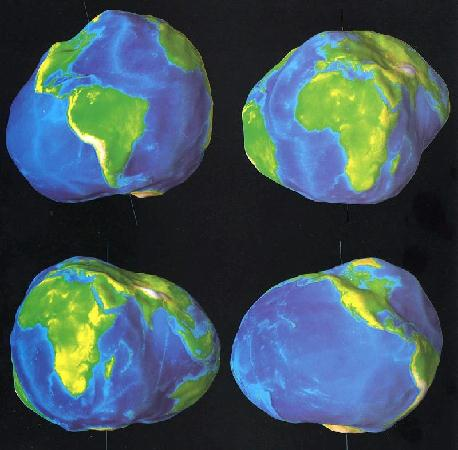
\includegraphics[height=6cm]{06.radionavegacion/Imagenes/forma-tierra.jpg}
      \label{fig:forma.tierra}} \subfigure[Amanecer de la Tierra, fotograf\'ia tomada por la 
    misi\'on \mbox{Apolo 8} (1968)]{
      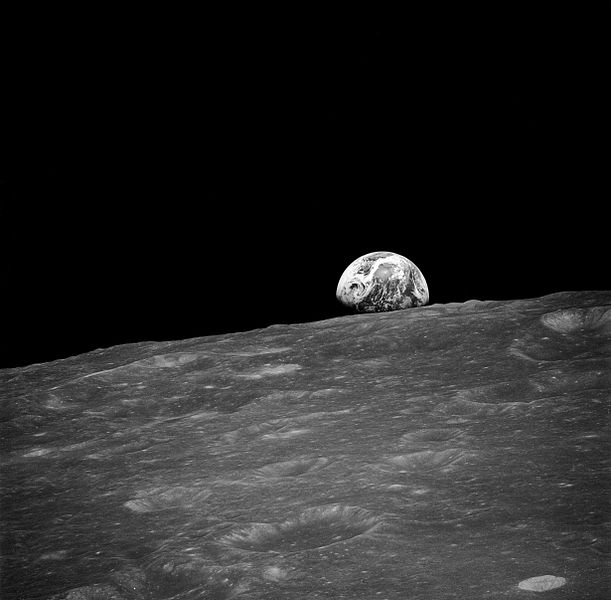
\includegraphics[height=6cm]{06.radionavegacion/Imagenes/amanecer-tierra.jpg}
      \label{fig:amanecer.de.la.tierra}}
    \subfigure[Dimensiones
    % \\ {\tiny (Fuente:
    % \url{http://www.kalipedia.com/geografia-general/tema/forma-dimensiones-tierra.html?x=20070417klpgeogra_6.Kes\&ap=1})}}
    ]{
      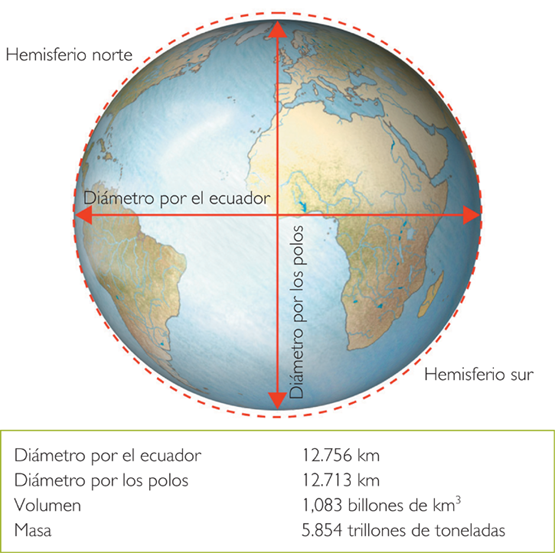
\includegraphics[height=6.5cm]{06.radionavegacion/Imagenes/dimensiones-tierra.png}
      \label{fig:dimensiones.tierra}} 

\subfigure[ Rotaci\'on ]{
      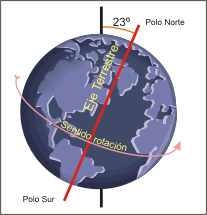
\includegraphics[height=5.5cm]{06.radionavegacion/Imagenes/RotacionTerrestre.png}
      \label{fig:rotacion.tierra}} 
\subfigure[ Precesi\'on ]{
      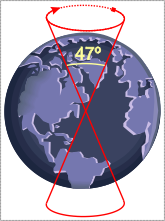
\includegraphics[height=5.5cm]{06.radionavegacion/Imagenes/Precesion.png}
      \label{fig:precesion.tierra}} 
\subfigure[ Nutaci\'on ]{
      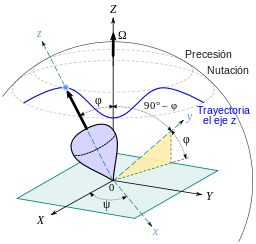
\includegraphics[height=5.5cm]{06.radionavegacion/Imagenes/nutacion.png}
      \label{fig:nutacion.tierra}} 
\subfigure[ Los movimientos
    \mbox{principales} ]{
      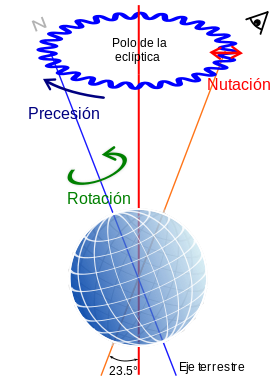
\includegraphics[height=5.5cm]{06.radionavegacion/Imagenes/rotacion-precession-nutation.png}
      \label{fig:los.tres.movimientos.tierra}}

    \caption{El planeta Tierra}
  \end{figure}

\end{landscape}


El planeta Tierra tiene los siguientes movimientos al desplazarse en el espacio:

\begin{itemize}
	\item \textbf{Movimiento de rotaci\'on:} Es un movimiento que efectúa la Tierra girando sobre sí misma a lo largo de un eje ideal denominado Eje Terrestre que pasa por sus polos. Una vuelta completa, tomando como referencia a las estrellas, dura 23 horas con 56 minutos y 4 segundos y se denomina ``\emph{día sid\'ereo}''. 



La primera referencia tomada por el ser humano fue el Sol, cuyo movimiento aparente originado en la rotación de la Tierra determina el día y la noche, dando la impresión que el cielo gira alrededor del planeta. En el uso coloquial del lenguaje se utiliza la palabra ``\emph{día}'' para designar este fenómeno, que en astronomía se refiere como \emph{día solar} y se corresponde con el tiempo solar.

Los 3 minutos y 56 segundos de diferencia se deben a que en ese plazo de tiempo la Tierra ha avanzado en su órbita y debe de girar algo más que un día sideral para completar un día solar, Figura \ref{fig:rotacion.tierra}.



El eje terrestre forma un ángulo de 23,5º respecto a la normal de la eclíptica, fenómeno denominado ``\emph{Oblicuidad de la Eclíptica}''. Esta inclinación produce largos meses de luz y oscuridad en los polos geográficos, además de ser la causa de las estaciones del año, causadas por el cambio del ángulo de incidencia de la radiación solar.

        \item \textbf{Movimiento de traslación:} Es un movimiento por el cual la Tierra se mueve alrededor del Sol. La causa de este movimiento es la acción de la gravedad, originándose cambios que, al igual que el día, permiten la medición del tiempo. Tomando como referencia el Sol, resulta lo que se denomina año tropical, lapso necesario para que se repitan las estaciones del año. Dura 365 días, 5 horas y 47 minutos. El movimiento que describe es una trayectoria elíptica de 930 millones de kilómetros, a una distancia media del Sol de prácticamente 150 millones de kilómetros ó 1 U.A. (Unidad Astronómica). De esto se deduce que la Tierra se desplaza con una rapidez media de 106200 km/h (29,5 km/s).

La trayectoria u órbita terrestre es elíptica. El Sol ocupa uno de los focos de la elipse y, debido a la excentricidad de la órbita, la distancia entre el Sol y la Tierra varía a lo largo del año. A primeros días de enero se alcanza la máxima proximidad al Sol, produciéndose el perihelio, donde la distancia es de 147,5 millones de km,; mientras que en los primeros días de julio se alcanza la máxima lejanía, denominado afelio, donde la distancia es de 152,6 millones de km.

\item \textbf{Movimiento de precesión:} 
también denominado precesión de los equinoccios, es debido a que la Tierra no es esférica, sino un elipsoide achatado por los polos. Si la Tierra fuera totalmente esférica, sólo realizaría los movimientos anteriormente descritos, Figura \ref{fig:precesion.tierra}.

Una vuelta completa de precesión dura 25767 años, ciclo que se denomina año platónico, cuya duración había sido estimada por los antiguos mayas.

\item \textbf{Movimiento de nutación:} debido al achatamiento de los polos y a la atracción de la Luna sobre el eje ecuatorial. También en un movimiento de vaivén y se produce durante el movimiento de precesión, este recorre a su vez una pequeña elipse (como si fuese una pequeña vibración). Una vuelta completa a la elipse suponen 18,6 años, lo que supone que en una vuelta completa de precesión la Tierra habrá realizado 1385 bucles, Figura \ref{fig:nutacion.tierra}.

\item \textbf{Bamboleo de Chandler:} pequeña oscilación del eje de rotación de la tierra que añade 0,7 segundos de arco en un período de 433 días a la precesión de los equinoccios. Fue descubierto por el astrónomo norteamericano Seth Carlo Chandler en 1891, y actualmente no se conocen las causas que lo producen, aunque se han propuesto varias teorías (fluctuaciones climáticas causantes de cambios en la distribución de la masa atmosférica, posibles movimientos geofísicos bajo la corteza terrestre, etc.)


\end{itemize}


\subsection{Coordenadas geogr\'aficas}
\label{sec:06.coordenadas.geograficas}

El sistema de coordenadas geogr\'aficas determina todas las posiciones de la superficie terrestre utilizando las dos coordenadas angulares de un sistema de coordenadas esf\'ericas que est\'a alineado con el eje de rotaci\'on de la Tierra. Este define dos \'angulos medidos desde el centro de la Tierra, ver Figura \ref{fig:latitud-longitud}:

\begin{itemize}
\item {\bf\Gls{latitud}:} mide el \'angulo entre cualquier punto y el ecuador. Las
  l\'ineas de latitud se llaman paralelos y son c\'irculos paralelos al
  ecuador en la superficie de la Tierra.

Debido a   que 
la insolaci\'on sobre la superficie terrestre depende de la latitud y dada la distancia que
  nos separa del Sol, los rayos luminosos que llegan hasta el planeta Tierra 
  son pr\'acticamente paralelos. La inclinaci\'on con que estos rayos
  inciden sobre la superficie de la Tierra es, pues, variable seg\'un la
  latitud. En la zona intertropical, a mediod\'ia, caen casi verticales,
  mientras que inciden tanto m\'as inclinados cuanto m\'as se asciende en
  latitud, es decir cuanto m\'as nos acercamos a los Polos. El las zonas donde ocurre este fen\'omeno se denominan tr\'opicos y se consideran dos paralelos notables con esta denominaci\'on: el tr\'opico de Cancer en el hemisferio Norte y el tr\'opico de Capricornio en el hemisferio Sur. %, ver Figura \ref{fig:tropico.cancer}.

As\'i se
  explica el contraste entre las regiones polares, muy fr\'ias y las
  tropicales, muy c\'alidas.


\item {\bf \Gls{longitud}:} mide el \'angulo a lo largo del ecuador desde cualquier   punto de la Tierra. Se acepta que Greenwich en Londres es la
  longitud 0 en la mayor\'ia de las sociedades modernas. Las l\'ineas de
  longitud son c\'irculos m\'aximos que pasan por los polos y se llaman
  meridianos.
\end{itemize}



\begin{figure}[!h]
  \centering
  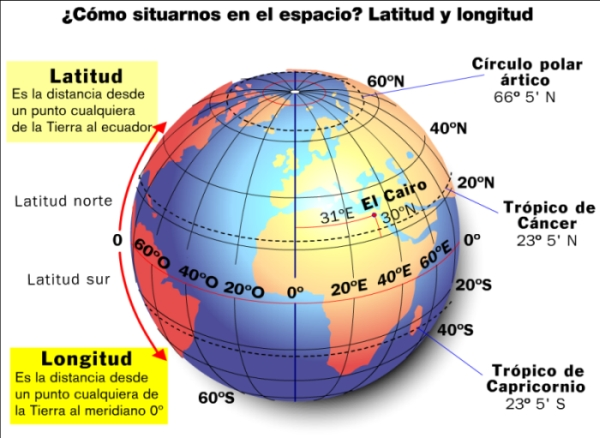
\includegraphics[width=\textwidth]{06.radionavegacion/Imagenes/latitud_longitud.jpg}
  \caption{Latitud y longitud}
  \label{fig:latitud-longitud}
\end{figure}

% \begin{figure}[!h]
%   \begin{minipage}[c]{0.50\linewidth}
%     \centering
%     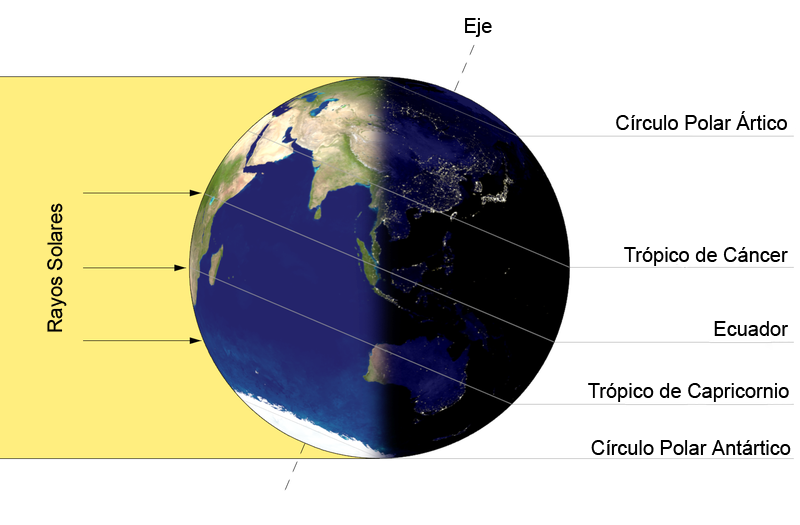
\includegraphics[width=0.95\textwidth]{06.radionavegacion/Imagenes/solsticio-diciembre.png}
%     \captionof{Tr\'opico de C\'ancer en el sosticio del mes de Junio,
%       {\scriptsize Fuente:
%         \url{https://www.lifeder.com/tropico-cancer/}}}
%     \label{fig:tropico.cancer}
%   \end{minipage}
%   \begin{minipage}[c]{0.50\linewidth}
Combinando estos dos \'angulos, se puede expresar la posici\'on de cualquier punto de la superficie de la Tierra. Por ejemplo, 
la ciudad de C\'ordoba en Argentina tiene coordenadas 31º 25' 0'' S, 64º 11' 0'' W lo que significa
latitud 31 grados 25 minutos 0 segundos Sud (desde el ecuador) y longitud 64 grados 11 minutos 0 segundos Oeste (desde Greenwich). 
As\'i un radio vector dibujado desde el centro de la tierra seg\'un estas coordenadas esf\'ericas pasar\'a por la mencionada ciudad de C\'ordoba.

El Ecuador es un elemento importante de este sistema de coordenadas, representa el cero de los \'angulos de latitud y el punto medio entre los polos. Es el plano fundamental del sistema de coordenadas geogr\'aficas.
    
%   \end{minipage}

% \end{figure}

Estas coordenadas usualmente se utilizan en planos de tipo proyecci\'on Mercator o en una \ac{UTM}. %, en el Ap\'endice \ref{sec:proyecciones.cartograficos} se describen con m\'as detalle estos tipos de proyecciones. 


 \section{Distancia, direcci\'on, tiempo, el Norte}
 \label{sec:distancia.direccion.tiempo}

 \subsection{Distancia}
 \label{sec:distancia}

 La distancia se mide como la longitud de la l\'inea que une a dos puntos, su unidad habitual para el uso en navegaci\'on es la \emph{\gls{nauticalmile}} (NM), la cual se define como 1 minuto de latitud o $6076$\,pies ($1852$\,m). A veces es necesario convertir de NM a \gls{statutemile} (SM) y viceversa, lo cual se hace de la siguiente forma:

\[\displaystyle
	\frac{\text{Millas estatutarias}}{\text{Millas n\'auticas}} 
	= \frac{76}{66}
\]

 Relacionado con el concepto de distancia se encuentra el de \emph{velocidad}, el cual indica la tasa de cambio de posici\'on. La velocidad se expresa usualmente en millas por hora (mph). Si la medida de la distancia es en NM, entonces la velocidad se expresa en \gls{nudo}. Una velocidad de 200 nudos es igual a una velocidad de 200 NM por hora.

Para calcular la distancia entre puntos sobre la superficie terrestre es necesario tener en cuenta no es plana, lo que implica que existir\'an ligeras (o grandes) distorsiones si se realiza esta operaci\'on sobre un mapa (dependiendo del tipo de este ultimo).
  
Adem\'as, el hecho de que la Tierra sea un geoide introduce variaciones
adicionales, que deber\'an  (o no) tenerse en cuenta dependiendo de la precisi\'on con que se desee realizar la medici\'on. 

A los fines de una primera aproximaci\'on, puede asumirse que la Tierra es esf\'erica.

Entre dos puntos cualesquiera de la superficie terrestre pueden trazarse líneas curvas diferentes: la ortodrómica, la loxodrómica. %y la isoazimutal.

\begin{description}
\item[Loxodr\'omica \label{loxodromica}] % (del griego  % \selectlanguage{greek} lox'oc
  % λοξóς
  %\selectlanguage{spanish}
  % ``oblicuo'' y \greektext dr'omoc
  % δρóμος
  %\latintext  ``carrera, curso'') 
  a la línea que une dos puntos cualesquiera de la
  superficie terrestre cortando a todos los meridianos con el mismo
  ángulo, ver Figura \ref{fig:loxodromica}. La loxodrómica, por tanto, es fácil de seguir manteniendo el
  mismo rumbo marcado por la brújula. Su representación en el mapa
  dependerá del tipo de proyección del mismo, por ejemplo en la de
  Mercator es una recta.

\item[Ortodrómica \label{ortodromica}] %(del griego \greektext enje'ia 
	% \latintext ``recto'' y
	% \greektext dr'omoc
 	% \latintext ''carrera'') 
	es el camino más corto entre dos puntos de la superficie terrestre; es el arco del círculo máximo que los une, menor de 180 grados, Figura \ref{fig:ortodromica}. 

% \item[Isoazimutal] La línea o curva isoazimutal, IsoZ($X,\theta$), es el lugar geométrico de los puntos sobre la superficie terrestre cuyo rumbo inicial ortodrómico respecto a un punto fijo $X$ es constante e igual a $\theta$.

% Es decir, si el rumbo inicial ortodrómico desde S hasta X es de 80 grados, la línea isoazimutal asociada es la formada por todos los puntos cuyo rumbo ortodrómico inicial al punto X es de 80º.
\end{description}

\begin{figure}[!h]
  \subfigure[Loxodr\'omica]{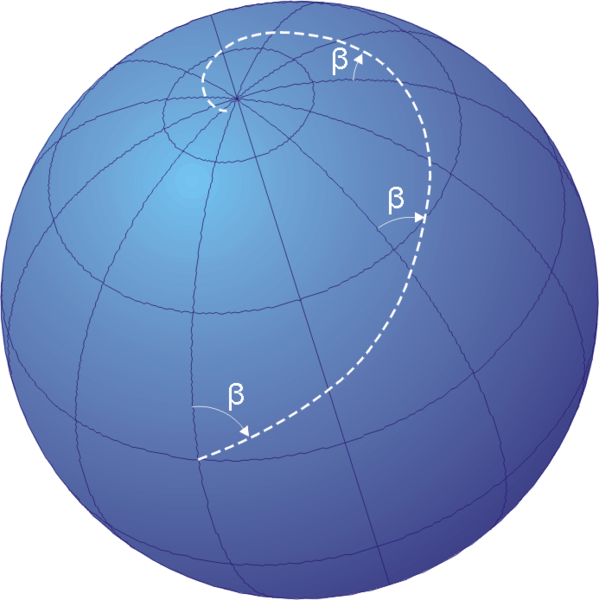
\includegraphics[height=5.8cm]{06.radionavegacion/Imagenes/loxodromica.png} \label{fig:loxodromica}}
  \subfigure[Ortodr\'omica]{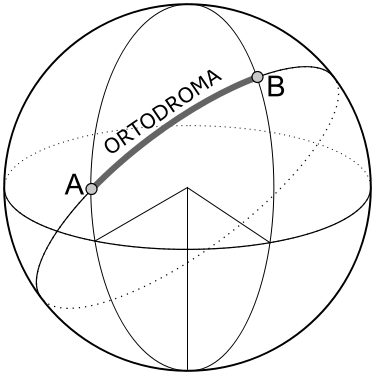
\includegraphics[height=5.8cm]{06.radionavegacion/Imagenes/ortodroma.png} \label{fig:ortodromica}}
  \subfigure[Comparaci\'on de ambas l\'ineas]{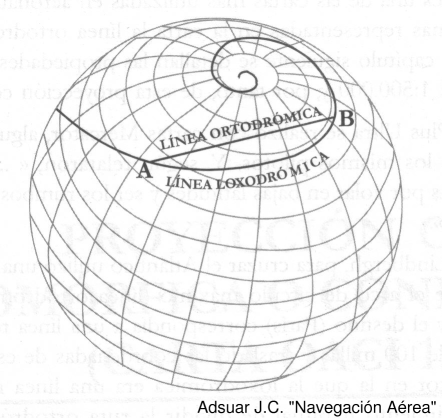
\includegraphics[height=5.8cm]{06.radionavegacion/Imagenes/comp-loxo-orto.png} \label{fig:ortodromica.loxodromica.comparacion}}
	\caption{Distancia entre dos puntos sobre la Tierra}
\end{figure}

Pedro Nunes, un geógrafo portugués, publicó en ``\emph{Tratado de la navegaci\'on}'' (1546) un descubrimiento con grandes implicaciones para la navegación. Antes de él se creía que marchando sobre la superficie terrestre con un rumbo fijo, es decir, formando un ángulo constante con la meridiana, la línea recorrida era un círculo máximo. Dicho con otras palabras, que un navío que siguiese este derrotero daría la vuelta al mundo y volvería al punto de partida. Nunes señaló la falsedad de este concepto al demostrar que la curva recorrida se va acercando al polo, alrededor del cual da infinitas vueltas, sin llegar nunca a él; o, dicho en lenguaje técnico, que tiene el polo por punto asintótico.

Una característica de la ortodrómica es que presenta un ángulo diferente con cada meridiano, (excepto cuando dicha ortodrómica coincide con un meridiano o con el ecuador). Esta característica representó un grave inconveniente para la navegación, solucionado hacia los últimos años del Siglo XX con el sistema GPS, porque antes del mismo, era difícil trazar una ruta de navegación que siguiera la ortodrómica ya que obligaría a continuos cambios de rumbo. 

\begin{minipage}[c]{0.5\linewidth}
Cuando las distancias eran grandes y seguir el camino más corto suponía un ahorro significativo, se realizaba una aproximación marcando una serie de puntos intermedios, en los cuales se cambiaba de rumbo y, de ésta manera, se lograba una aproximación a las correspondientes loxodrómicas.

  Un concepto interesante que relaciona las l\'ineas ortodr\'omicas y
  las millas n\'auticas es que sobre las mismas se puede calcular la
  distancia entre dos puntos. Por ejemplo, dados los puntos A y B
  sobre una de estas curvas, ver Figura
  \ref{fig:Distancia.entre.dos.puntos.esfera.terrestre.tikz}.  El
  ángulo entre los radio vectores que parten del centro de la esfera y
  terminan en cada uno de estos puntos es 30º 25'. Convirtiendo este
  \'angulo a minutos se obtiene 1825', como 1' = 1 NM, sobre la esfera
  que representa al planeta Tierra la distancia entre los puntos A y B
  es de 1825 NM.
\end{minipage}\hspace{0.05\linewidth}
\begin{minipage}[c]{0.4\linewidth}
  \begin{center}
    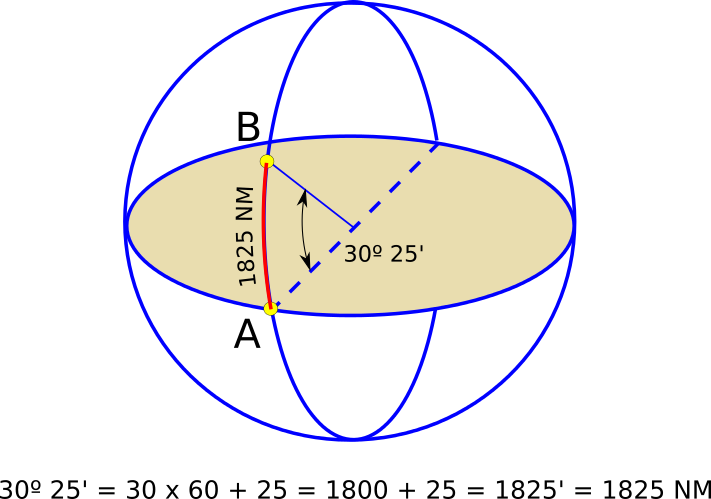
\includegraphics[width=0.9\linewidth]{06.radionavegacion/Imagenes/06.00.navegacion/06_milla_nautica.png}
	\captionof{figure}{
Distancia entre dos puntos sobre la Tierra. 
Adaptado de \protect\cite{Tooley_Aircraft_communications_and_navigation_systems}
}
    \label{fig:Distancia.entre.dos.puntos.esfera.terrestre.tikz}
\end{center}

  \end{minipage}



\subsection{Direcci\'on}
\label{sec:direccion}

La direcci\'on es la posici\'on de un punto en el espacio relativo a otro sin referencia a la distancia entre ellos. En la navegaci\'on se utiliza un sistema n\'umerico para indicar la direcci\'on como el mostrado en la Figura \ref{fig:rosa.de.compas}. En la misma se divide la vista en planta en 360º, comenzando con el norte a 0º y continuando en sentido de las agujas del reloj, pasando por el este a 90º, sur 180º y oeste 270º, volviendo al norte.

Este c\'irculo se denomina rosa de comp\'as, las l\'ineas cuasi-verticales de la Figura \ref{fig:rosa.de.compas} son meridianos. Por el punto A pasa el meridiano a trav\'es de 000º y 180º de la rosa, el punto B se encuentra en una direcci\'on de 60º respecto del A y el punto C en una direcci\'on de 220º del punto A.

\subsubsection{Definiciones}
\label{sec:definiciones.navegacion}

\begin{description}

\item [Trayectoria] (trayectory) se define como el conjunto de puntos del espacio por los cuales pasa la aeronave durante su vuelo (ver Figura \ref{fig:trayectoria}).

\item [Ruta] es la curva resultante de proyectar la trayectoria sobre la superficie de la Tierra (ver Figura \ref{fig:trayectoria}).

\item [Waypoints] son puntos conocidos a lo largo de la ruta, y a menudo resaltan por alguna raz\'on en particular (Lugares de reporte obligatorio, puntos de intersecci\'on de aerov\'ias, etc.) (ver Figura \ref{fig:trayectoria}).

\item [Tramo] (leg) se define como un segmento de ruta comprendido entre dos waypoints (ver Figura \ref{fig:trayectoria}). 

\begin{figure}[!h]
  \centering
  \subfigure[Rosa de comp\'as]{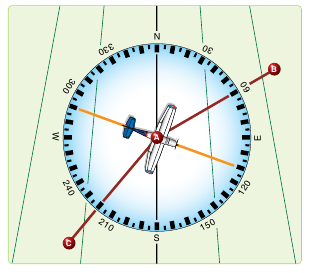
\includegraphics[height=6.7cm]{06.radionavegacion/Imagenes/rosa.png}  \label{fig:rosa.de.compas}}
  \subfigure[Trayectoria, ruta, Fuente \protect\cite{Salazar_nav_aerea}]{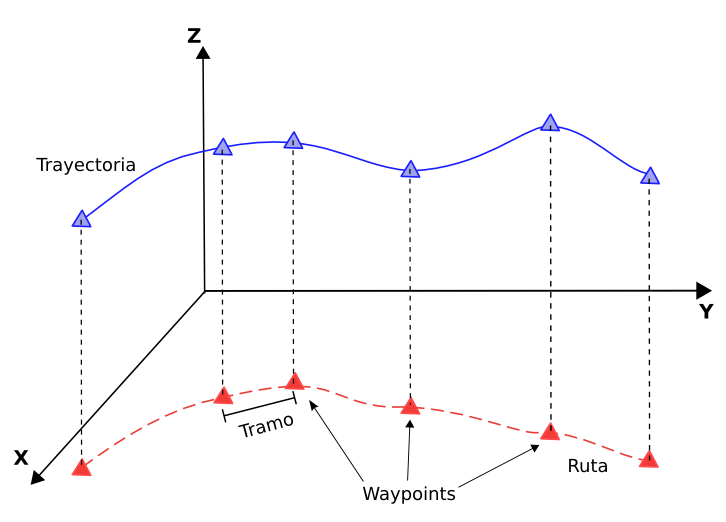
\includegraphics[height=6.7cm]{06.radionavegacion/Imagenes/trayectoria-ruta.png}  \label{fig:trayectoria}} 

  \caption{Elementos de navegaci\'on}
\end{figure}


  \item[Rumbo] el rumbo o o ``Heading'' (HDG) es el \'angulo entre el norte y el eje   longitudinal de la aeronave (hacia donde apunta su nariz). No
  coincide necesariamente con el vector velocidad (Track) dado que es
  posible, por ejemplo, que el piloto modifique el rumbo para
  contrarestar un viento cruzado (ver Figura \ref{fig:curso}).

\item [Curso deseado] es el \'angulo entre el norte (cualquiera que se est\'e usando: magn\'etico, geogr\'afico, etc) y la l\'inea recta que une dos waypoints sucesivos en la ruta. En ingl\'es se denomina ``\textit{Desired Track}'', y se abrevia DTK (ver Figura \ref{fig:curso}).

\item [Derrota] En n\'autica, la derrota es el trayecto que ha recorrido una embarcaci\'on desde un punto ``\textit{A}'' hasta otro punto ``\textit{B}''. En el derrotero o carta n\'autica se traza la ruta a seguir; contiene informaciones importantes para el navegante, tales como ubicaci\'on de faros, boyas, profundidad del agua, etc. En navegaci\'on a\'erea es el \'angulo entre el norte y la l\'inea tangente a la ruta (dicha tangente corresponde, por cierto, al vector velocidad de la aeronave). En ingl\'es se le llama ``\textit{Track}'' o TK (ver Figura \ref{fig:curso}).

\item [Error transversal] El error transversal o ``\textit{Cross-Track Error}'' (XTE) es la distancia perpendicular entre la posici\'on de la aeronave y la l\'inea que representa al curso deseado. \footnote{Es conveniente tener en cuenta que la diferencia entre el curso deseado (DTK) y la ruta realmente seguida (TK) por lo general es producida por factores externos tales como el viento cruzado (en el caso de las aeronaves) o las corrientes marinas (si se habla de barcos).}

\end{description}

\begin{figure}[!h]
  \centering
  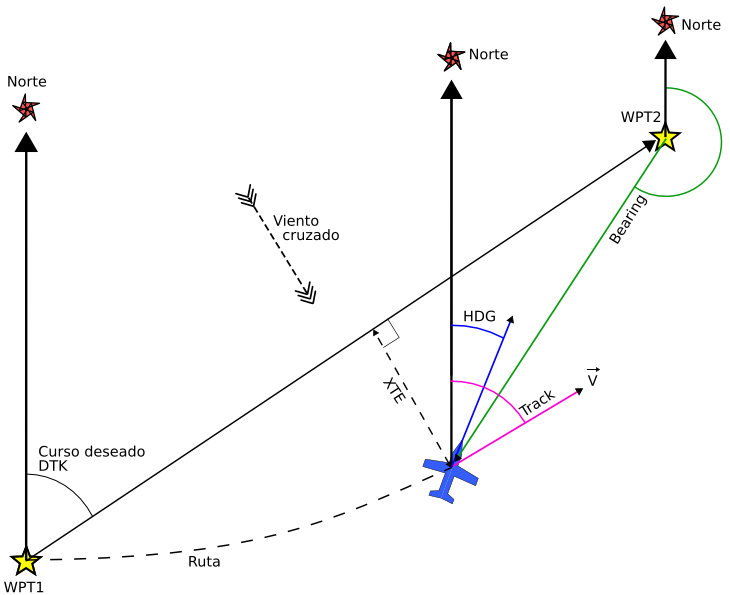
\includegraphics[keepaspectratio,height=10cm]{06.radionavegacion/Imagenes/curso-derrota-rumbo-marcacion.png}  
  \caption{Elementos de navegaci\'on (continuaci\'on),  Fuente \protect\cite{Salazar_nav_aerea}}
  \label{fig:curso}
\end{figure}

\subsection{Tiempo}
\label{sec:tiempo}

La navegaci\'on a\'erea es un problema de cuatro dimensiones: latitud, longitud, altura y es necesario saber \emph{en qu\'e momento} estuvimos (o estaremos) en una posici\'on dada.

Muchos de los sistemas de navegaci\'on modernos est\'an basados en la medici\'on de intervalos de tiempo.

La medici\'on del tiempo se encuentra asociada a la historia del calendario, esto es, un modo sistem\'atico de organizar los d\'ias en semanas, meses, a\~nos y milenios.

 Una de las formas m\'as sencillas es con referencia a las fases de la Luna, el calendario de este tipo es denominado \emph{lunar} y el tiempo entre repeticiones de una fase dada de la Luna (p.e., luna nueva) es denominado \emph{mes sin\'odico}. Este dura, en promedio, $29.530589$ d\'ias.

 El calendario lunar tiene como ventaja que posee una referencia muy f\'acil de seguir, pero tiene como inconveniente que el mes sin\'odico no tiene un n\'umero entero de d\'ias.

 Por otra parte, las estaciones del a\~no son fen\'omenos muy importantes para la vida humana, pero las fases de la Luna son independientes de estas. Por ese motivo algunas culturas prefirieron marcar el paso del tiempo siguiendo el movimiento aparente del Sol por el cielo, cuya trayectoria se denomina ecl\'iptica\footnote{El movimiento que realiza la Tierra en torno al Sol (traslación), genera un plano al que se le ha dado el nombre de Eclíptica. Como el eje de giro de la Tierra tiene una inclinación promedio de 23º 27', entonces el Ecuador terrestre y la eclíptica forma entre si, este mismo ángulo.\\La proyección de la Eclíptica sobre la Esfera Celeste, forma un círculo máximo que se encuentra inclinado con respecto a ella, 23º 27'.
\\
 La incidencia perpendicular de los haces de luz solar, barren casi 47º (exactamente 46º 54') sobre el globo terráqueo. Cuando inciden a 23º 27' Latitud Norte, alcanzan el denominado Trópico de Cáncer (21 de Junio). Cuando inciden a 23º 27' Latitud Sur, el Trópico de Capricornio. Estos son los puntos máximos y mínimos que alcanzará el Sol en su desplazamiento imaginario por el cielo. Estos puntos reciben el nombre de Solsticios, del latín Solstitium, que significan ``\emph{el Sol más lejos}''. Los nombres de los Trópicos están determinados por las constelaciones de Cáncer, en el Hemisferio Norte del la Esfera Celeste y de Capricornio, en el Sur.
\\
De manera similar, existen dos puntos en donde se interceptan el Ecuador Celeste y la Eclíptica. Estos son el Punto Vernal  ubicado en la constelación de Los Peces (Piscis) y el Punto Otoñal (d) ubicado en la constelación de La Virgen (Virgo). El Punto Vernal representa en las coordenadas celestes lo que el Meridiano de Greenwich en las coordenadas terrestres, es decir el punto origen de las coordenadas celestes.
\\
En estos dos puntos, los haces de luz solar inciden perpendicularmente sobre el Ecuador de la Tierra, iluminando de manera uniforme a todo el planeta. Estos puntos reciben el nombre de Equinoccios, del latín Aequus Nox, que significa “igual duración de las noches”. En su recorrido anual, la Tierra alcanza estos puntos el 21 de marzo y 21 de Septiembre, respectivamente. }. Este calendario se denomina \emph{solar}, y el tiempo transcurrido entre dos pasos suscesivos del Sol por el equinoccio de primavera es denominado \emph{a\~no vernal equinoxial} y tiene una duraci\'on de $365.2424$ d\'ias.

 Se comprob\'o que  19 a\~nos vernales equinoxiales equivalen a $234.997$ meses sin\'odicos ($\approx 235$), lo que implica que cada 19 a\~nos las fases de la Luna y sus fen\'omenos asociados (eclipses) caen casi ex\'actamente en la misma fecha. Este ciclo es denominado \emph{met\'onico} en honor al astr\'onomo Met\'on, siglo V a. C.

 Posteriormente los romanos establecieron un calendario que, tras sucesivas adaptaciones, evolucion\'o al calendario actualmente utilizado en el hemisferio occidental, el calendario Gregoriano.

 La medici\'on del tiempo tiene, actualmente, dos familias:
 \begin{itemize}
       \item Las asociadas al movimiento de los cuerpos celestes
       \item Las basadas en las oscilaciones de los \'atomos
 \end{itemize}

\subsubsection{Tiempo solar}
\label{sec:tiempo.solar}

El tiempo solar es una medida del tiempo fundamentada en el movimiento aparente del Sol sobre el horizonte del lugar. Toma como origen el instante en el cual el Sol pasa por el Meridiano, que es su punto más alto en el cielo, denominado mediodía.1 A partir de este instante se van contando las horas en intervalos de 24 partes hasta que completan el ciclo diurno.

Sin embargo, el Sol no tiene un movimiento regular a lo largo del año, y por esta razón el tiempo solar se divide en dos categorías:

\begin{itemize}
\item {\bf Tiempo solar verdadero} está basado en el día solar verdadero,
  el cual es el intervalo entre dos regresos sucesivos del Sol al
  meridiano. Puede ser medido con un reloj de sol, y se corresponde
  con el amanecer, el mediodía o el anochecer: se basa en lo que es
  posible observar de manera directa. Con un reloj de sol adecuadamente orientado se puede marcar este tiempo, Figura \ref{fig:reloj.de.sol}.

La duración de un día solar verdadero varía a lo largo del año. Esto se debe a que la órbita terrestre es una elipse, con lo cual la Tierra en su movimiento de traslación se mueve más veloz cuando se acerca al Sol y más despacio cuando se aleja de él. Debido a esto, el día solar más corto es el 15 de septiembre, mientras que el día solar más largo es el 22 de diciembre, tanto el Hemisferio Norte como en el Hemisferio Sur.


\item \textbf{ Tiempo solar medio} está basado en un sol ficticio que viaja a una   velocidad constante a lo largo del año, y es la base para definir el
  día solar medio (24 horas u $86400$ segundos). Se corresponde con el
  tiempo civil y se coordina mediante el Tiempo Medio de Greenwich.
\end{itemize}


La diferencia entre el tiempo solar verdadero y el tiempo solar medio, que en ocasiones llega a ser de 15 minutos, es llamada \emph{Ecuación de tiempo}, Figura \ref{fig:2012.ecuacion.del.tiempo}.


\begin{figure}[!h]
  \centering
  \subfigure[Reloj de sol]{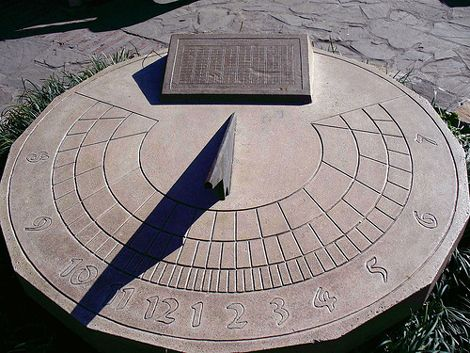
\includegraphics[height=6.5cm]{06.radionavegacion/Imagenes/reloj-de-sol.jpg} \label{fig:reloj.de.sol}}
  \subfigure[Ecuaci\'on del tiempo, a\~no 2012]{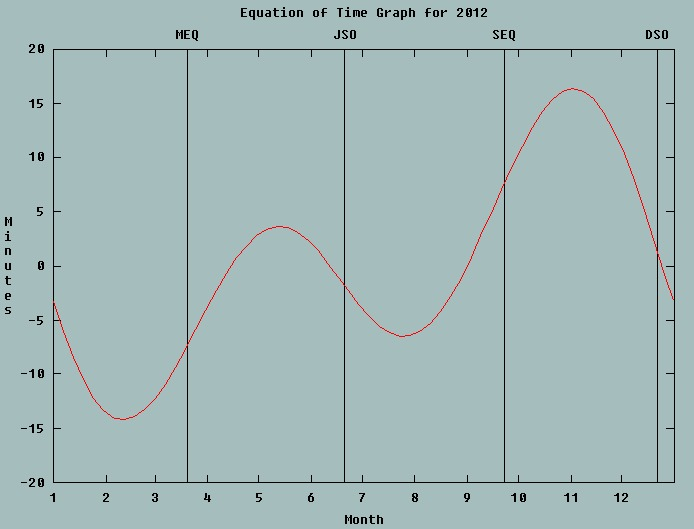
\includegraphics[height=6.5cm]{06.radionavegacion/Imagenes/2012-ecuacion-tiempo.jpg} \label{fig:2012.ecuacion.del.tiempo}}

  \subfigure[Meridiano de Greenwich]{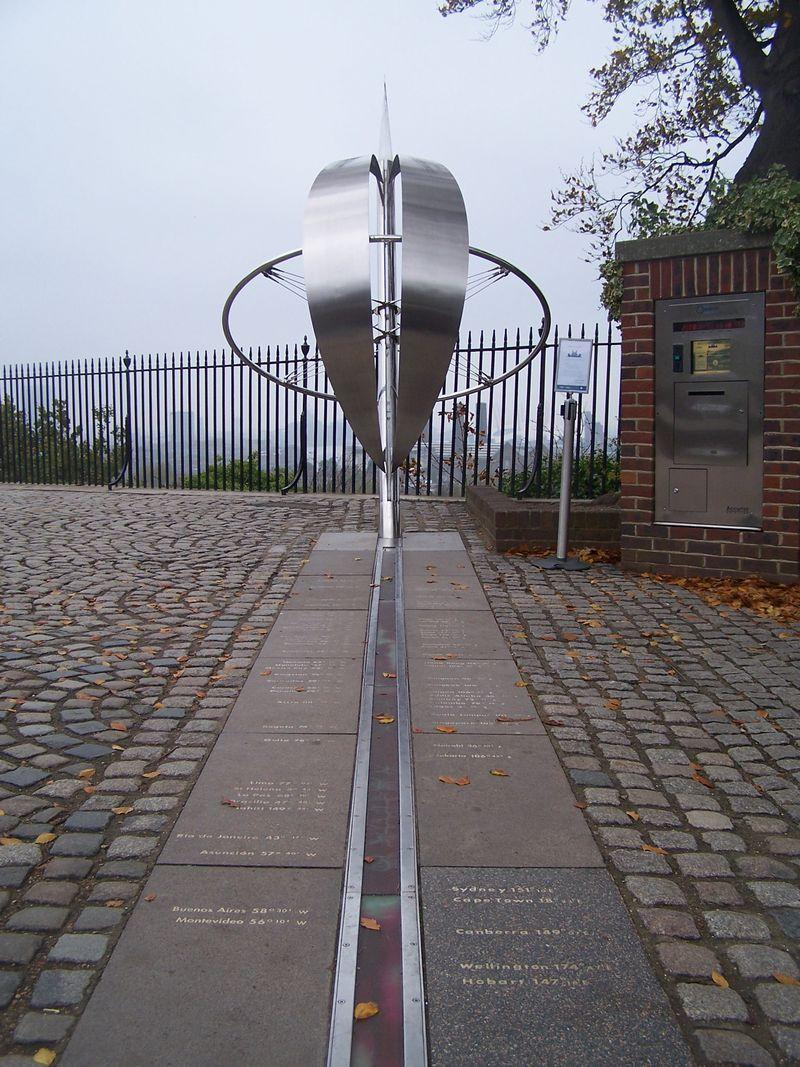
\includegraphics[height=6.5cm]{06.radionavegacion/Imagenes/Greenwich-Meridian-Line.jpg} \label{fig:meridiano.greenwich}}
  \subfigure[Primer reloj at\'omico (1948)]{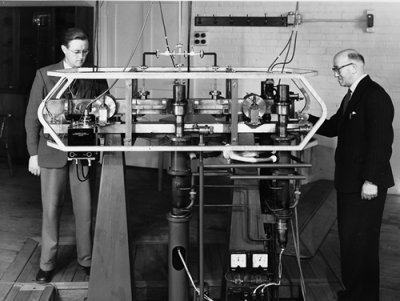
\includegraphics[height=6.5cm]{06.radionavegacion/Imagenes/TAI.jpg} \label{fig:primer.reloj.atomico}}

  \caption{Medici\'on del tiempo}
\end{figure}

\subsubsection{ Greenwich Mean Time}
\label{sec:greenwich.mean.time}

El  Greenwich Mean Time (GMT)  es una escala de tiempo basada en el paso
del Sol Medio por el meridiano de Greenwich (espec\'ificamente por el viejo
Observatorio Real de Greenwich, que es el punto de referencia).
Este tiempo est\'a  obsoleto pues en 1928 la Uni\'on Astron\'omica 
 Internacional introdujo el  Universal Time (UT) para reemplazarlo.

\subsubsection{Tiempo Universal (UT)}
\label{sec:tiempo.universal}

El UT reemplaz\'o al GMT puesto que este \'ultimo se basaba en la medici\'on de la posici\'on del Sol, y existen problemas asociados a la medici\'on precisa de la misma.

El UT se basa en la medici\'on de la posici\'on de referencias astron\'omicas, como los cu\'asares, consigui\'endose mayor precisi\'on.

 A pesar de su mayor precisión el UT sigue siendo una escala de tiempo no uniforme, pues en el fondo se basa en la medición del período de rotación del planeta y éste presenta anomalías. De hecho, en 1956 el Comité Internacional de Pesos y Medidas decidió que la definición del segundo se haría en función del período de revolución de la Tierra para una época dada, y así el segundo de efemérides fue definido como:

La fracción 1/31556925,9747 del año tropical medio para el 1ro. de Enero de 1900 a las 12 horas.

Debido a la existencia de las mencionadas anomalías, existen varios tipos de UT:
\begin{description}

\item [UT0:] Es el Tiempo Universal definido mediante observaciones de
  puntos de referencia astronómicos. Inicialmente era medido mediante
  relojes de péndulo, pero conforme la tecnología de los relojes fue
  avanzando, se notó la existencia de errores.


\item [UT1:] Cuando a UT0 se le aplican las correcciones debidas al
  movimiento de los polos (efecto Chandler y otros) obtenemos
  UT1. Esta escala es la más ampliamente utilizada por los astrónomos
  y a menudo el término UT se refiere a ella.


\item [UT2:] Debido a que la velocidad de rotación de la Tierra no es
  constante, UT1 presenta variaciones estacionales relacionadas, entre
  otras cosas, a las mareas y el intercambio de energía entre la
  Tierra y la atmósfera. Al aplicar las correcciones debidas a las
  variaciones más fuertes y regulares (del orden de 3 milisegundos por
  día), obtenemos UT2. Esta escala, la más precisa para el Tiempo
  Universal, sigue siendo irregular y por ello ha caído en desuso
  después de la aparición de nuevos métodos no astronómicos para la
  medición del tiempo.
\end{description}


\subsubsection{ Temps Atomique International (TAI)}
\label{sec:temps.atomique.international}

 Dado que las escalas de tiempo anteriores no eran suficientemente regulares, se desarrollaron relojes cada vez más precisos que permitieron desligarse de la rotación de la Tierra como patrón que definía el tiempo. Estas investigaciones desembocaron en el reloj atómico, que marca el tiempo examinando el comportamiento de los átomos de un material dado, y por tanto la escala de tiempo así construida no depende (o depende muy poco) de factores externos.

 \begin{myboxAzul}{}
   Desde mediados de 1950 se empezaron a desarrollar relojes atómicos
   suficientemente precisos y por ello la 13ra. Conferencia General de
   Pesos y Medidas celebrada en el año 1967 pudo definir el segundo
   del Sistema Internacional como: \vspace{3mm}
   % \fbox{\parbox{\textwidth}

   {\it La duración de $9192631770$ períodos de la onda de la
     radiación emitida por el átomo de Cesio 133 cuando se realiza la
     transición entre los dos niveles hiperfinos del estado
     fundamental del átomo.}
%}
\end{myboxAzul}
%\vspace{3mm}

En función de esta definición, la BIPM (Oficina Internacional de Pesos y Medidas), localizada en París, Francia, coordina y promedia los datos provenientes de un gran número de relojes atómicos alrededor del globo para generar una escala de tiempo uniforme llamada TAI (Tiempo Atómico Internacional). 



\subsubsection{Tiempo Universal Coordinado (UTC)}
\label{sec:tiempo.universal.coordinado}
 El UTC es una escala de tiempo atómica internacional ampliamente utilizada en el ámbito civil. De hecho, hoy en día prácticamente todos los países del mundo definen sus horas locales en función de UTC6.9, añadiendo o restando un número entero de horas según convenga a su localización geográfica.

En cierta forma, UTC puede verse como la manera de reconciliar el tiempo atómico (TAI) con el tiempo dado por la rotación de la Tierra  UT1.

\begin{myboxAzul}{}
  El UTC tiene la misma frecuencia del TAI pero cada cierto tiempo se le
  añaden (o sustraen) segundos extras (llamados ``leap seconds'') para
  mantenerlo sincronizado dentro de $\pm 0.9$ s de UT1. De esta
  manera, se obtiene la exactitud del tiempo atómico sin divorciarse
  completamente del fenómeno de la rotación terrestre.
\end{myboxAzul}

%Los ``leap seconds'' empezaron a usarse el 30 de Junio de 19726.10, y habitualmente se introducen al final del último minuto del último día de diciembre o del último día de junio, si hace falta. Hasta el momento se han introducido 33 segundos, todos ellos de retraso.

\subsubsection{Tiempo GPS (GPST)}
\label{sec:tiempo.gps}


También llamado GPST, el tiempo GPS es el utilizado como referencia para las aplicaciones relacionadas con el sistema de posicionamiento global por satélite del Departamento de Defensa de los EE.UU.

El GPST es un tiempo de naturaleza atómica que no es alterado por ``leap seconds''. Toma como época de origen las 00:00 UTC de la noche del 5 al 6 de enero de 1980. Dado que para esa fecha se habían introducido 19 ``leap seconds'', la siguiente expresión es válida:

\[ TAI - GPST = 19 s
\]

\begin{myboxAzul}{}
  Un concepto adicional importante es la llamada {\it semana
    GPS}. Ésta empieza la noche del sábado al domingo, de modo tal que
  el 17 de marzo del 2004 correspondió a la semana GPS 1262. Las
  semanas GPS tienen un ciclo de 1024, y el primer ciclo se alcanzó en
  la noche del 21 al 22 de Agosto de 1999, llamado ``{\it GPS Week Rollover}''.
\end{myboxAzul}

\subsubsection{Tiempo Loran-C}
\label{sec:tiempo.loran.c}

%El término LORAN, que significa ``Long Range Navigation'' (Navegación de Largo Alcance), co\-rres\-pon\-de a una cadena de transmisores de radiofrecuencia de amplio alcance que permiten conocer con cierta precisión (aproximadamente 0,25 NM) la posición de un receptor sobre la superficie terrestre.

Los transmisores pertenecientes a la cadena (o ``chain'', en inglés) Loran poseen relojes atómicos que están sincronizados entre sí. Estos relojes no son alterados por ``leap seconds'', lo que hace que se separe progresivamente de UTC.

\begin{myboxAzul}{}
  La época de inicio de los relojes atómicos del sistema Loran-C fue
  las 0hs del 1 de enero de 1958.
\end{myboxAzul}


 \subsection{El Norte}
 \label{sec:el.norte}
 El concepto de ``\emph{Norte}'' engloba una serie de definiciones que es necesario conocer y diferenciar adecuadamente:

\begin{itemize}
\item\textbf{ Norte geográfico: }Es el que viene dado por la intersección del eje de rotación de la Tierra con la superficie de la misma. Es llamado también ``Norte verdadero'', y en él confluyen todos los meridianos.

\item \textbf{Norte magnético:} Es el punto donde la mayor parte de las líneas de fuerza del campo magnético terrestre entran en la superficie. Se puede detectar utilizando instrumentos tales como la brújula y la v\'alvula de flujo (flux valve).

Existe una denominaci\'on similar para los polos ubicados en el hemisferio Sur.

Es importante hacer notar que los polos geográfico y sus correspondientes  magnéticos \textbf{NO} coinciden, y que además los polos magnéticos cambian su posición con el tiempo, ver Figura \ref{fig:06.movimiento.polos.magneticos}.

\begin{figure}[!htb]
  \centering
  \subfigure[Movimientos polo norte magn\'etico]{\includegraphics[width=0.45\textwidth]{06.radionavegacion/Imagenes/06.00.navegacion/06_polo_norte_movimientos_00.gif}}
  \subfigure[Movimientos polo sur magn\'etico]{\includegraphics[width=0.45\textwidth]{06.radionavegacion/Imagenes/06.00.navegacion/06_polo_sur_movimientos.gif}}
  \caption{Movimiento de los polos magn\'eticos \protect\cite{MovimientoPolosMagneticos} 
}
%{\scriptsize Fuente \url{http://wdc.kugi.kyoto-u.ac.jp/poles/polesexp.html\#Fig1}}

  \label{fig:06.movimiento.polos.magneticos}
\end{figure}

\item \textbf{Declinación magnética:} Es el ángulo de desviación entre las posiciones del norte magnético y geográfico, vistas desde un punto en particular. Se denota como D y se considera positiva cuando el ángulo medido está hacia el Este del norte verdadero, y negativo en caso contrario. 

Lo anterior significa que si sobre un punto de la superficie terrestre la brújula marca un rumbo de 115º, y sabemos que la declinación magnética en ese punto es 4º E, el rumbo verdadero serán 119º. 

En la Figura \ref{fig:declinacion-magnetica} se representa la declinación magnética para dos puntos diferentes de la superficie terrestre. Note que en uno de ellos la geometría es tal que la declinación es cero. 

\begin{figure}[!h]
    \centering
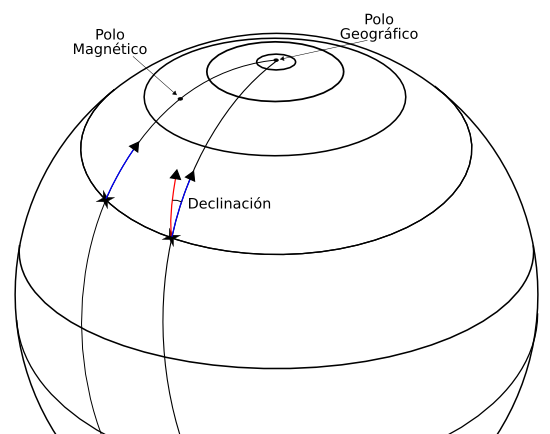
\includegraphics[keepaspectratio,width=0.6\textwidth]{06.radionavegacion/Imagenes/declinacion-magnetica.png}
\caption{Declinaci\'on magn\'etica en dos puntos diferentes de la Tierra. Fuente  \protect\cite{Salazar_nav_aerea}}
\label{fig:declinacion-magnetica}
\end{figure}

\item \textbf{Líneas isógonas:} Se llaman así a las líneas que, sobre las cartas de navegación o los mapas, unen puntos que tienen la misma declinación magnética. Son también denominadas Líneas Isogónicas. Adicionalmente, si una línea corresponde a puntos con declinación 0º, se habla de Línea Agónica. 

\item \textbf{Norte de la Brújula:} Es el norte magnético tal y como lo indica a bordo el instrumento adecuado (brújula o flux valve). No indica realmente el norte magnético pues el instrumento comete errores por diversas razones (presencia de masas metálicas cercanas, líneas de campo magnético que no son horizontales, etc).

\item \textbf{Desviación magnética:} Es el error angular cometido por la brújula o flux valve. El fabricante de la aeronave puede corregirla hasta cierto punto.

La Figura \ref{fig:declinacion-desviacion} presenta la relación entre los nortes geográfico, magnético y de la brújula con sus correspondientes diferencias angulares.

\begin{figure}[!htb]
    \centering
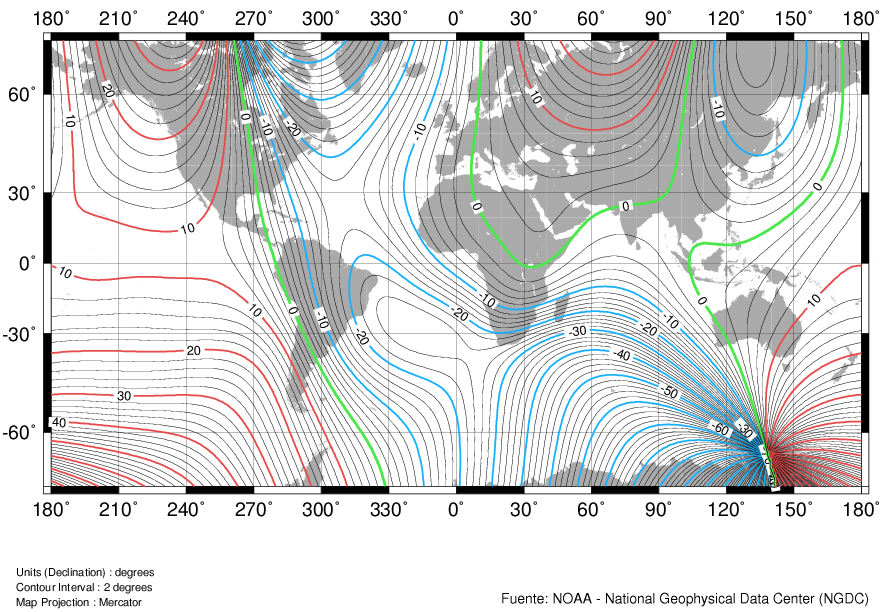
\includegraphics[keepaspectratio,width=\textwidth]{06.radionavegacion/Imagenes/declinacion-magnetica-anio-2000.png}
\caption{Declinaci\'on magn\'etica - A\~no 2000. Fuente \protect\cite{Salazar_nav_aerea}}
\label{fig:declinacion-magnetica-anio-2000}
\end{figure}

\begin{figure}[!htb]
    \centering
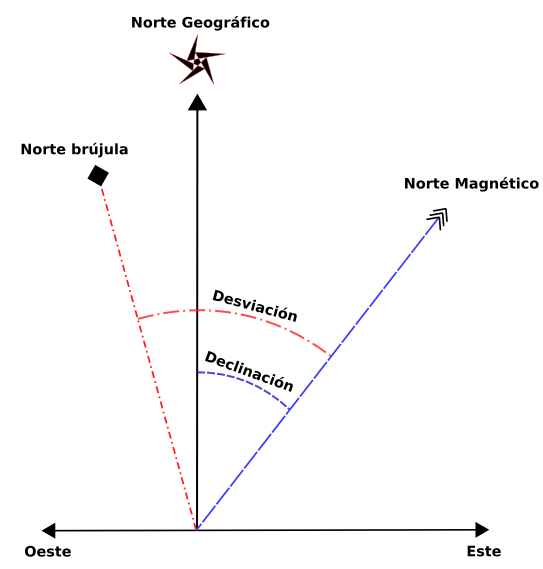
\includegraphics[keepaspectratio,width=0.6\textwidth]{06.radionavegacion/Imagenes/declinacion-desviacion.png}
\caption{Los diferentes nortes y sus diferencias angulares. Fuente \protect\cite{Salazar_nav_aerea}}
\label{fig:declinacion-desviacion}
\end{figure}


\item \textbf{Norte de la Cuadrícula:} Cuando se navega a grandes latitudes (muy al norte o muy al sur del planeta), no tiene sentido guiarse por el norte magnético debido, entre otras cosas, a las grandes declinaciones implicadas.

Es por ello que se define arbitrariamente el Norte de la Cuadrícula como el norte indicado por los meridianos de la carta de navegación que se está usando para navegar. 
\end{itemize}




\section{Cartas de navegaci\'on aeron\'autica}
\label{sec:cartas.navegacion.aeronautica}

La carta aeron\'autica se define como la representaci\'on de una porci\'on de la tierra, su relieve y construcciones, dise\~nada especialmente para satisfacer los requisitos de la navegaci\'on a\'erea. Se trata de un mapa en el que se reflejan las rutas que deben seguir las aeronaves, y se facilitan las ayudas, los procedimientos y otros datos imprescindibles para el piloto.

El gran problema asociado a la construcción y utilización de cartas es que la superficie de la Tierra \textbf{no se puede representarse con fidelidad en ninguna carta}. Esto se debe a que una esfera \emph{no es una superficie desarrollable}, es decir, no es posible convertirla a un plano sin generar distorsiones. Es el mismo problema que enfrentaríamos si intentáramos convertir la cáscara de una naranja en un plano sin alterarla, Figura \ref{fig:comparacion.proyecciones.cartograficas}. 

Superficies que sí son desarrollables son los cilindros y los conos. En ambos casos, basta con cortar dichas superficies por un lugar conveniente y seguidamente las podemos estirar sin deformarlas y convertirlas en planos.

Por esta razón, la práctica común al construir una carta consiste en proyectar la superficie de la Tierra sobre una de estas tres superficies (plano, cono o cilindro). Dicha proyección consiste en escoger un conjunto de reglas geométricas y aplicarlas sistemáticamente a toda la superficie que se interesa proyectar, Figura \ref{fig:proyecciones.cartograficas}.

% \subsection{Proyecciones cartogr\'aficas}
% \label{sec:proyecciones.cartograficas}

% Como las cartas de navegación son proyecciones de la superficie terrestre, es conveniente estudiar primero las características de las proyecciones para entender luego las de las cartas. 

%  Existe un gran número de tipos diferentes de proyecciones según el conjunto de reglas que se escojan para hacerla (por ejemplo: punto de origen, tipo de superficie de proyección, posición de la superficie, etc.). Cada uno de estos conjuntos de reglas introduce diferentes tipos de distorsiones, que son inevitables, y en base a éstas se puede a su vez definir diferentes propiedades de la proyección.

% \begin{figure}[!h]
%   \centering
%   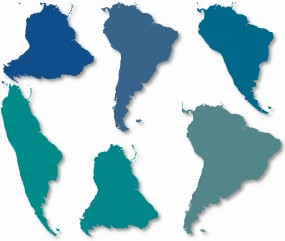
\includegraphics[width=0.8\textwidth]{06.radionavegacion/Imagenes/comparacion-proyecciones.jpg}
%   \caption{Am\'erica del Sur en diferentes proyecciones. ¿Cu\'al es la correcta? \\{\footnotesize Fuente: \url{http://www.progonos.com/furuti/MapProj/Normal/TOC/cartTOC.html}}}
%   \label{fig:comparacion.proyecciones.cartograficas}
% \end{figure}


% La razón de que existan tantos tipos de proyecciones diferentes es que estas propiedades las hacen adecuadas para un uso u otro, según lo que se desee. En las siguientes secciones estudiaremos las propiedades más importantes que pueden tener las proyecciones, y por ende, las cartas hechas con ellas. 

% \begin{figure}[!h]
%   \centering
%   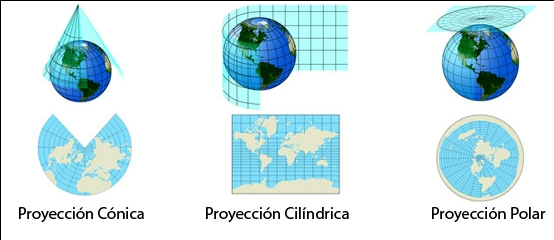
\includegraphics[width=\textwidth]{06.radionavegacion/Imagenes/proyecciones.jpg}
%   \caption{Proyecciones cartogr\'aficas}
%   \label{fig:proyecciones.cartograficas}
% \end{figure}

% Entre las propiedades de las proyecciones se tiene:

% \begin{description}
% \item[Conformidad] Un mapa conforme es aquél que preserva los ángulos (y por tanto, las formas) a nivel local. Esto significa que las formas de características tales como deltas, ríos, etc. son reconocibles, pues la distorsión que sufren no es grande.
% \item[Equivalencia] Una proyección es equivalente o autálica si mantiene las proporciones entre las áreas representadas. Esto quiere decir que si un país dado A tiene el doble del área que un país B, en una proyección equivalente dicha proporción se mantiene, Figura \ref{fig:groenlandia.africa.comparacion.superficies.segun.tipo.proyeccion}. 

% Las proyecciones equivalentes o autálicas son de escasa utilidad para la navegación, pero por otra parte son muy útiles cuando se quiere presentar información que ha de compararse a simple vista, como población, producción industrial, etc., o para elaborar atlas escolares.


% \begin{figure}[!h]
%   \centering
%   \subfigure[Proyeccion Mercator]{
%   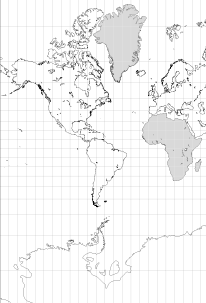
\includegraphics[height=7cm]{06.radionavegacion/Imagenes/merEqTh.png}
%   \label{fig:proyeccion.mercator.groenlandia.africa}
%   }
%   \subfigure[Proyeccion Mollweide]{
%   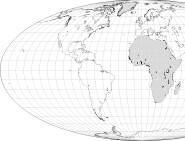
\includegraphics[height=7cm]{06.radionavegacion/Imagenes/mollEqTh.png}
%   \label{fig:proyeccion.mollweide.groenlandia.africa}
%   }
%   \caption{Comparaci\'on de las superficies de Groenlandia y \'Africa seg\'un el tipo de proyecci\'on utilizada, superficie \'Africa = 29800000\,km$^2$, superficie Groenlandia = 2175600\,km$^2$\\{\footnotesize Fuente: \url{http://www.progonos.com/furuti/MapProj/Normal/CartProp/AreaPres/areaPres.html}}
% }
%   \label{fig:groenlandia.africa.comparacion.superficies.segun.tipo.proyeccion}
% \end{figure}


% \item[Equidistancia] Una proyección es equidistante cuando posee un conjunto bien definido y completo de líneas a lo largo de las cuales la escala se mantiene constante, Figura \ref{fig:proyeccion.equidistante}.

% Al indicar que posee un conjunto bien definido y completo de líneas, nos referimos al hecho de que muchas proyecciones tienen unas pocas líneas a lo largo de las cuales la escala se mantiene constante (a menudo llamadas líneas automecoicas. No obstante, en las cartas equidistantes el número de líneas que tienen esta propiedad es mucho más grande.

% Por ejemplo, es posible crear una carta con una proyección equidistante que esté centrada en una ciudad dada A, y entonces se podría calcular con exactitud la distancia entre tal ciudad A y cualquier otra ciudad que se represente en la carta.

% Las cartas equidistantes a menudo distorsionan mucho los ángulos y áreas, y por ello tienen una utilidad limitada. Sin embargo es posible obtener pocas distorsiones si el área representada es pequeña. 

%     \begin{figure}[!h]
%       \centering
%   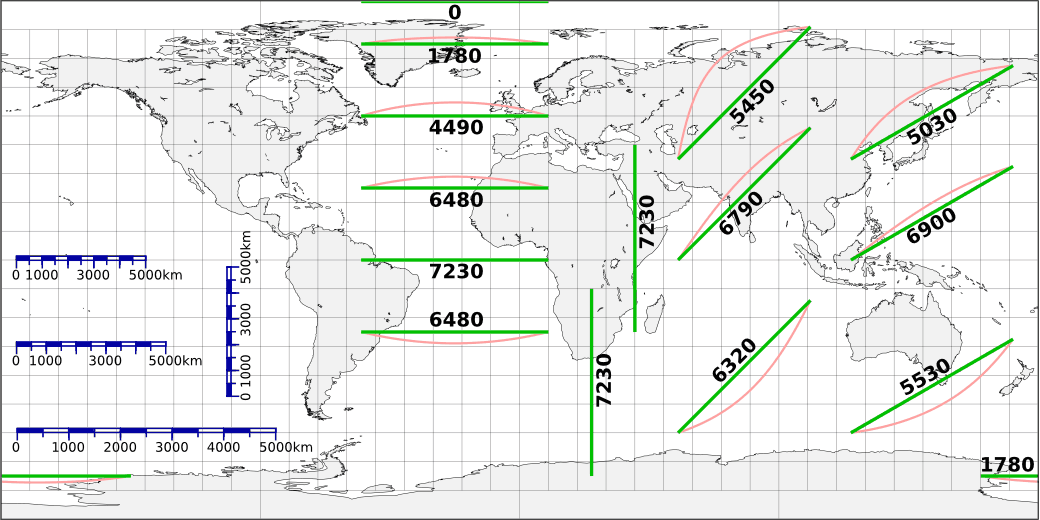
\includegraphics[height=9cm]{06.radionavegacion/Imagenes/proyeccion-equidistante.png}
%       \caption{Proyecci\'on equidistante cil\'indrica, distancias en km. Cada escala gr\'afica es v\'alida a lo largo de su propio paralelo. Solo la escala vertical es v\'alida en cualquier lugar.\\{\footnotesize Fuente: \url{http://www.progonos.com/furuti/MapProj/Normal/CartProp/AreaPres/areaPres.html}}}
%       \label{fig:proyeccion.equidistante}
%     \end{figure}


% \item[Dirección]  Otra propiedad importante de las proyecciones es la referida a si distorsionan, y de qué manera, las direcciones. Por ejemplo, una proyección que muestra de forma correcta todas las direcciones desde su centro a cualquier otro punto de la carta se llama azimutal.

% Hay al menos dos maneras diferentes de entender la dirección: En función del círculo máximo y en función del rumbo, y ambas maneras definen líneas muy importantes: 

% \begin{description}
% 	\item[Líneas Loxodrómicas] ver  \fullref{loxodromica}
% 	\item[Líneas Ortodrómicas] ver \fullref{ortodromica}
% \end{description}

% En la Figura \ref{fig:comparacion.entre.loxodromas.y.ortodromas} puede observarse una comparaci\'on entre este tipo de l\'ineas al conectar dos puntos.

% \begin{figure}[!h]
%   \centering
%   \subfigure[Proyecci\'on Mercator]{
% 	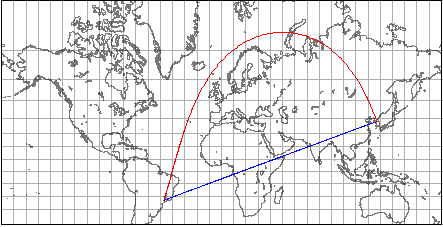
\includegraphics[height=6cm]{06.radionavegacion/Imagenes/gr-mr-s70-n80-s-40.png}
% 	}
%   \subfigure[Proyecci\'on polar azimutal equidistante]{
% 	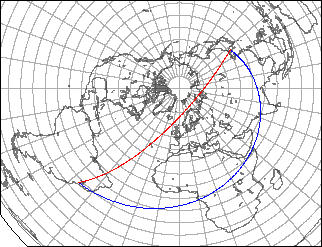
\includegraphics[height=6cm]{06.radionavegacion/Imagenes/gr-aze-s70.png}
% 	}
%   \subfigure[Proyecci\'on Lagrange]{
% 	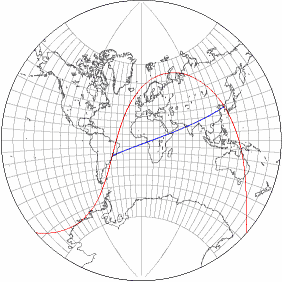
\includegraphics[height=6cm]{06.radionavegacion/Imagenes/lg-s70h.png}
% 	}
%   \caption{Comparaci\'on entre loxodromas y ortodromas, azul loxodromica, rojo ortodromica \\{\footnotesize Fuente: \url{http://www.progonos.com/furuti/MapProj/Normal/ShapePres/shapePres.html}}}
%   \label{fig:comparacion.entre.loxodromas.y.ortodromas}
% \end{figure}

% \end{description}

% \subsection{Las cartas OACI \cite{Salazar_nav_aerea}}

% La seguridad de la navegaci\'on a\'erea exige la elaboraci\'on y publicaci\'on de cartas aeron\'auticas actualizadas y precisas, que respondan a las necesidades actuales de la aviaci\'on. En consecuencia, corresponde a cada Estado miembro de la Organizaci\'on de Aviaci\'on Civil Internacional (OACI) adoptar las disposiciones necesarias para facilitar el esfuerzo de cooperaci\'on que supone la producci\'on y difusi\'on de cartas aeron\'auticas. Adem\'as, cada Estado tiene la obligaci\'on de proporcionar informaci\'on del propio territorio a trav\'es de las cartas aeron\'auticas.

% La Organizaci\'on de Aviaci\'on Civil Internacional (OACI), en su Anexo 4 - Cartas Aeron\'auticas, ha publicado una serie de normas y m\'etodos recomendados para la elaboraci\'on de las mismas. Adicionalmente, y como complemento y ayuda para la puesta en pr\'actica de estas normas, tambi\'en proporciona el Manual de Cartas Aer\'onauticas.

% Seg\'un la OACI, el dise\~no de las cartas aeron\'auticas debe tomar en cuenta una serie de factores, entre los cuales se pueden mencionar:

% \begin{itemize}

% \item  Debe utilizarse una proyecci\'on com\'un.

%   \item Las escalas utilizadas deben tener valores f\'acilmente
%   comprensibles.

%   \item Debe facilitarse la transici\'on de una carta a otra durante el
%   vuelo mediante una adecuada selecci\'on de alturas, construcciones u
%   otra informaci\'on relativa al terreno.

%   \item Deber\'ian publicarse simult\'aneamente las cartas que tienen conexi\'on
%   entre s\'i, ya sean cartas nuevas o sus revisiones.

% \end{itemize}

% \begin{landscape}
%   \newcommand{\minitab}[2][1]{\begin{tabular}{#1}#2\end{tabular}}
Cartas opcionales. Las seis cartas opcionales se producir\'an si, en opinión de las Autoridades aeron\'auticas de los Estados, contribuyen a la seguridad, regularidad y eficacia de las operaciones de las aeronaves.

Cartas condicionales. Las cinco cartas condicionales se producir\'an solamente si se cumplen determinadas condiciones o circunstancias.

\begin{table}%[!h]
  \centering
  \caption{Cartas aeron\'auticas OACI}
  \label{tab:cartas.aeronauticas.OACI}
  \begin{small}
    \begin{tabular}{|m{0.12\textheight}|m{0.4\textheight}|c|c|c|m{0.35\textheight}|}
      \cline{3-5} 
	\multicolumn{2}{c|}{} & %\multirow{2}*[1.5cm]{
      \begin{turn}{90}
        \textbf{Obligatoria}
      \end{turn}
      % }
      &%\multirow{2}*[1.5cm]{
      \begin{turn}{90}
        \textbf{Opcional}
      \end{turn}
      % }
      &%\multirow{2}*[1.5cm]{
      \begin{turn}{90}
        \textbf{Condicional \,}
      \end{turn}
      % } 
      & \multicolumn{1}{c}{}
      \\ \cline{1-2}\cline{6-6}
      \centering \textbf{Grupo} & \centering \textbf{Carta} & 
      & & &\multicolumn{1}{c|}{\textbf{Requerimientos}}\\ \hline

      \multirow{4}{0.12\textheight}{ Planificaci\'on previa al vuelo} &
      \parbox{\linewidth}{1. Plano de obst\'aculos de aeródromo – Tipo A \\
      (limitadores de utilización).} 
	&\cellcolor{red} & & &
       Aeródromos con obst\'aculos destacados en las \'areas de despegue y aterrizaje.
	\\
&&&&& \\
&&&&& \\
&&&&& \\

%       \multirow{4}{0.12\textwidth}{ Planificaci\'on previa al vuelo} &
%       \minitab[l]{1. Plano de obst\'aculos de aeródromo – Tipo A \\
%       \quad (limitadores de utilización).} &\cellcolor{red} & & &
%        Aeródromos con obst\'aculos destacados en las \'areas de despegue y aterrizaje.
% 	\\
%       &
%       2. Plano de obst\'aculos de aeródromo – Tipo B. & &\cellcolor{blue} & & \\
%       &
%       3. Plano de obst\'aculos de aeródromo – Tipo C.& & &\cellcolor{green} & \\
%       &
%       4. Carta topogr\'afica para aproximaciones de precisión. &\cellcolor{red} & & & Obligatoria en pistas con aproximaciones de precisión categorías II y III\\ \hline
%       \multirow{4}{0.12\textwidth}{ En vuelo} &
%       5. Carta de navegación en ruta. &\cellcolor{red} & & & 
% 	Zonas en las que se hayan establecido Regiones de Información de Vuelo (FIR)	\\
%       &
%       6. Carta de \'area. & & &\cellcolor{green} & \\
%       &
%       7. Carta de salida normalizada – Vuelo por instrumentos (SID). & & &\cellcolor{green} & \\
%       &
%       8. Carta de llegada normalizada – Vuelo por instrumentos (STAR). & & &\cellcolor{green} & \\
%       &
%       9. Carta de aproximación por instrumentos. &\cellcolor{red} & & &
% Aeródromos en los que se haya establecido tal tipo de aproximación \\
%       &
%       10. Carta de aproximación visual.  & & &\cellcolor{green} & \\ \hline
%       \multirow{4}{0.12\textwidth}{Movimientos en tierra %de 
%         %	las aeronaves en el aeródromo
%       } &
%       11. Plano de aeródromo/helipuerto &\cellcolor{red} & & & 
% En todos los que se utiliza regularmente la aviación civil internacional\\
%       &
%       12. Plano de aeródromo para movimientos en tierra.  & &\cellcolor{blue} & & \\
%       &
%       13. Plano de estacionamiento y atraque de aeronaves.  & &\cellcolor{blue} & & \\ \hline
%       \multirow{4}{0.12\textwidth}{Navegación a\'erea visual, trazado de posiciones, planificación} &
%       14. Carta aeron\'autica mundial (escala 1:1.000.000). & \cellcolor{red}& & & En todas las zonas especificadas por la OACI\\
%       &
%       15. Carta aeron\'autica (escala 1:500.000).  & &\cellcolor{blue} & & \\
%       &
%       16. Carta de navegación aeron\'autica (escala peque\~na). & &\cellcolor{blue} & & \\
%       &
%       17. Carta de posición.  & &\cellcolor{blue} & & \\ \hline

    \end{tabular}
  \end{small}
\end{table}
% \end{landscape}

% \subsubsection{Cartas OACI obligatorias}

% El Anexo 4 exige que cada pa\'is garantice la disponibilidad de seis (6) 
% tipos diferentes de cartas aeron\'auticas que se consideran obligatorias:

% \begin{enumerate}

% \item   Plano de obst\'aculos de aer\'odromo - OACI, Tipo A: Para aquellos
%   aer\'odromos donde hay obst\'aculos destacados en el \'area de la
%   \gls{trayectoria} de despegue.

%   \item. Carta topogr\'afica para aproximaciones de precisi\'on - OACI: Para
%   todos los aer\'odromos con pistas de aproximaci\'on de precisi\'on de
%   Categor\'ias II y III.

%   \item Carta de navegaci\'on en ruta - OACI: Para todas las zonas donde se
%   hayan establecido regiones de informaci\'on de vuelo (FIR).

%   \item Carta de aproximaci\'on por instrumentos - OACI: Para aquellos
%   aer\'odromos donde se hayan establecido procedimientos de aproximaci\'on
%   instrumentales.

%   \item Plano de Aer\'odromo/Helipuerto - OACI: Necesario para todos
%   aquellos aer\'odromos/helipuertos regularmente utilizados por la
%   aviaci\'on civil internacional.

%   \item Carta aeron\'autica mundial - OACI, 1:1 000 000: Publicada de
%   acuerdo a lo indicado en el Ap\'endice 5 del Anexo 4.
% \end{enumerate}

% \subsubsection{Cartas OACI condicionales}

% Adicionalmente a las anteriores, existen cinco cartas de publicaci\'on condicional, lo que significa que han de presentarse determinadas circunstancias para su publicaci\'on:

% \begin{description}

% \item [Plano de obst\'aculos de aer\'odromo - OACI, Tipo C] Necesario s\'olo
%   si en el AIP\footnote{Una publicación de información aeronáutica, más conocida por las siglas AIP (del inglés: Aeronautical Information Publication), es una publicación editada por las autoridades competentes en aviación civil (o por quien estas designen) que contiene información aeronáutica de carácter escencial para la navegación aérea. Se diseñan para que sean un manual que contenga detalles de leyes, procedimientos operativos, servicios disponibles o cualquier otra información que necesite una aeronave que sobrevuele el país en particular al que se refiere el AIP.}
%  no se publican los datos sobre obst\'aculos que requieren
%   los explotadores para generar sus procedimientos.

%   \item [Carta de \'area - OACI] Requerida si las rutas o los requisitos de
%   notificaci\'on de posici\'on son complicados y no pueden indicarse
%   adecuadamente en la carta habitual para ello (Carta de navegaci\'on en
%   ruta - OACI).

%   \item [Carta de salida normalizada - vuelo por instrumentos - OACI]
%   Llamadas cartas SID, se publican cuando existe una salida
%   normalizada de este tipo y no se pueda indicar con la claridad
%   suficiente en la Carta de \'area - OACI.

%   \item [Carta de llegada normalizada - vuelo por instrumentos - OACI]
%   Estas son las cartas STAR y se publican cuando existe una llegada
%   normalizada y no se pueda indicar con la claridad suficiente en la
%   respectiva Carta de \'area - OACI.

%   \item [Carta de aproximaci\'on visual - OACI] Necesaria para aquellos
%   aer\'odromos en los que se cumple al menos una de las siguientes
%   condiciones:

%   \begin{itemize}
%   \item  S\'olo existen instalaciones y servicios de navegaci\'on limitados.

%     \item No existen servicios de radiocomunicaciones.

%     \item No existen cartas a escala 1:500 000 del aer\'odromo y sus
%     alrededores.

%     \item Se han establecido procedimientos de aproximaci\'on visual.
%   \end{itemize}

% \end{description}

% \subsubsection{Cartas OACI opcionales}

% Finalmente, existen otras seis cartas denominadas opcionales porque la OACI delega a las autoridades de cada pa\'is la decisi\'on sobre su publicaci\'on si consideran que estas cartas contribuir\'an a la seguridad, regularidad y eficiencia de las operaciones a\'ereas.

% Tales cartas opcionales son:

% \begin{enumerate}
% \item \textbf{Plano de obst\'aculos de aer\'odromo - OACI, Tipo B:} Se publica
%   como ayuda para determinar las alturas cr\'iticas en alg\'un
%   procedimiento.

% \item  \textbf{Plano de aer\'odromo para movimientos en tierra - OACI:} Se
%   publica s\'olo cuando en el Plano de Aer\'odromo/Helipuerto - OACI
%   no puede indicarse con suficiente claridad los datos necesarios para
%   el movimiento de aeronaves en las calles de rodaje.

% \item  \textbf{Plano de estacionamiento y atraque de aeronaves - OACI: }Publicado
%   cuando, por la complejidad del terminal a\'ereo, no puede se\~nalarse en
%   el Plano de Aer\'odromo/Helipuero - OACI ni en el Plano de
%   aer\'odromo para movimientos en tierra - OACI suficiente
%   informaci\'on con respecto al estacionamiento de las aeronaves.

% \item  \textbf{Carta aeron\'autica - OACI 1:500 000:} Cuando los requisitos para la
%   navegaci\'on visual indiquen que puede sustituir o complementar a la
%   Carta aeron\'autica mundial - OACI, 1:1 000 000.

% \item  \emph{Carta de navegaci\'on aeron\'autica - OACI, escala peque\~na:} Igual
%   que la anterior.

% \item \textbf{ Carta de posici\'on - OACI:} Son cartas \'utiles para mantener un
%   registro continuo de la posici\'on de una aeronave en vuelo sobre
%   zonas oce\'anicas o escasamente pobladas.
% \end{enumerate}

% \subsubsection{La carta OACI 1:500 000}

% Esta carta est\'a basada en la llamada proyecci\'on c\'onica conforme de Lambert, que es una proyecci\'on c\'onica normal secante. La proyecci\'on superpone un cono sobre la esfera de la Tierra, con dos paralelos de referencia secantes al globo e intersec\'andolo. Esto minimiza la distorsi\'on proveniente proyectar una superficie tridimensional a una bidimensional. La distorsi\'on es m\'inima a lo largo de los paralelos de referencia, y se incrementa fuera de los paralelos elegidos. Como el nombre lo indica, esta proyecci\'on es conforme.

% Los pilotos utilizan estas cartas debido a que una l\'inea recta dibujada sobre una carta cuya proyecci\'on es conforme c\'onica de Lambert muestra la distancia verdadera entre puntos. Sin embargo, los aviones deben volar rutas que son arcos de c\'irculos m\'aximos para recorrer la distancia m\'as corta entre dos puntos de la superficie, que en una carta de Lambert aparecer\'a como una l\'inea curva que debe ser calculada en forma separada para asegurar de identificar los puntos intermedios correctos en la navegaci\'on.

% Es ampliamente utilizada para la navegaci\'on a\'erea visual, consider\'andose una de las cartas b\'asicas por proporcionar informaci\'on visual a una escala adecuada.

% \begin{figure}[!h]
%   \centering
%   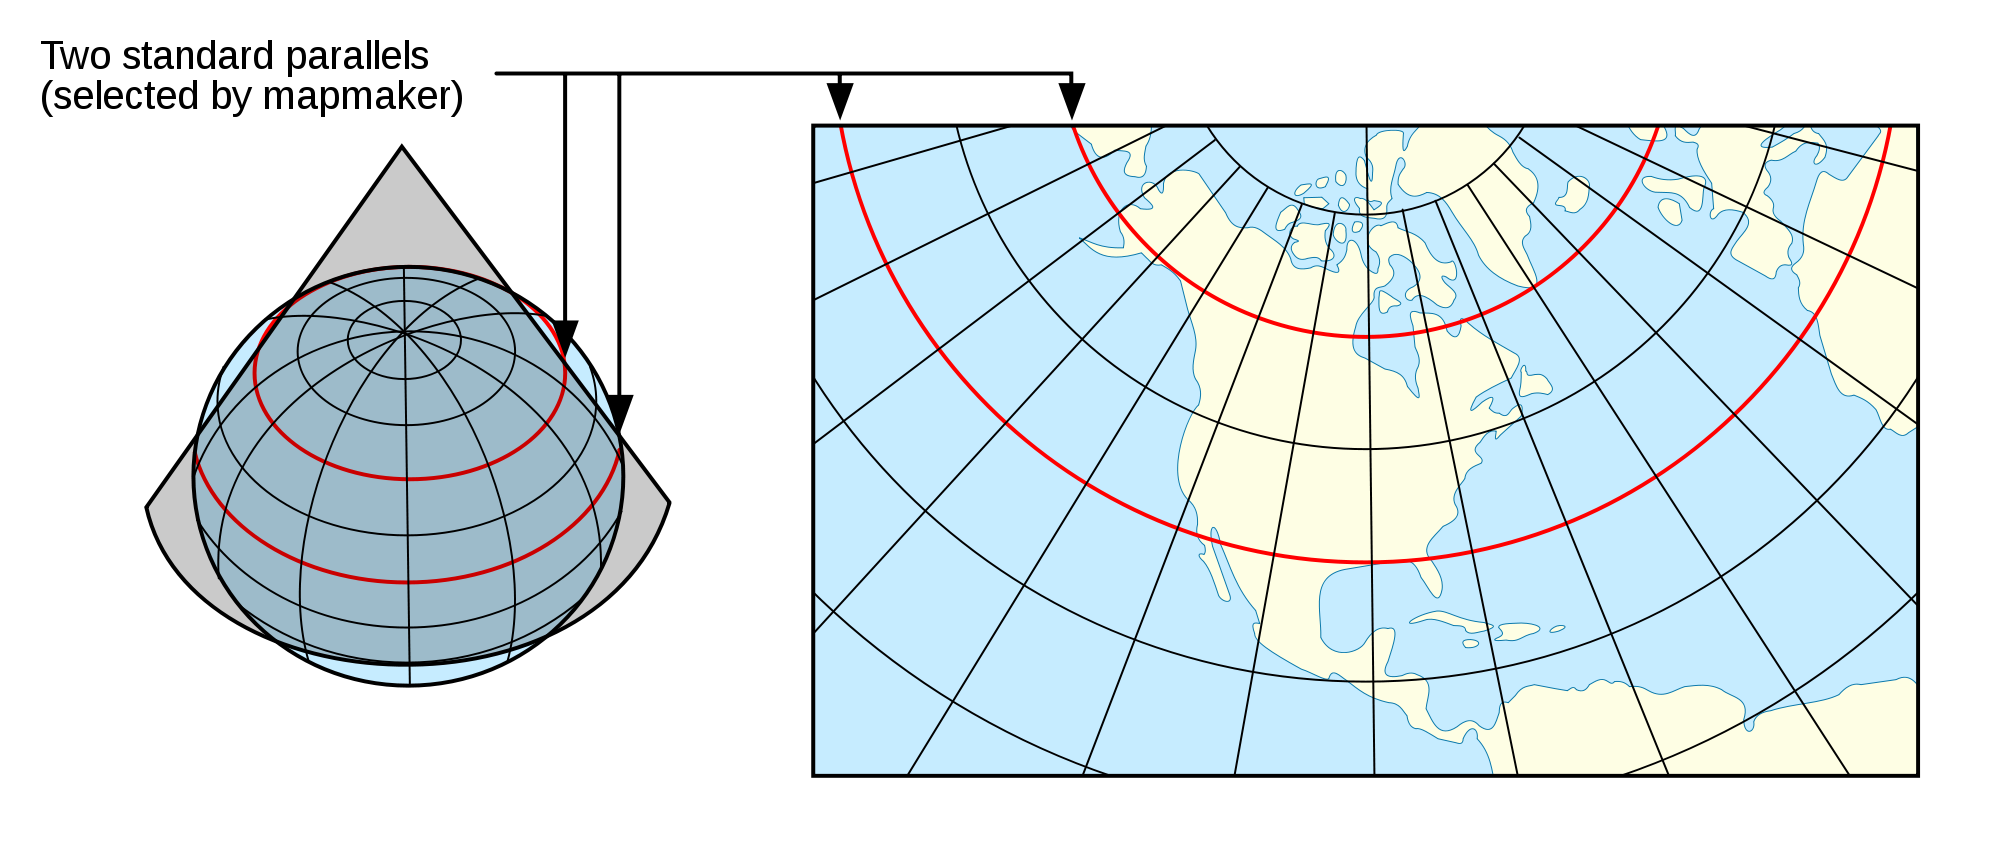
\includegraphics[height=8cm]{Imagenes/06.00.navegacion/2000px-Lambert_conformal_conic.png}
% %  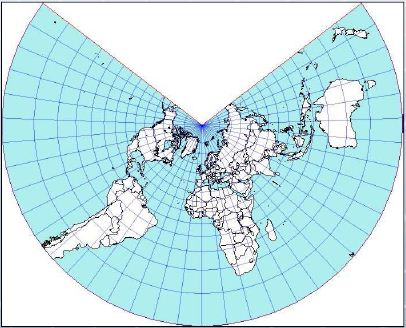
\includegraphics[height=8cm]{Imagenes/06.00.navegacion/proy_conica_lambert.jpg}
%   \caption{Proyecci\'on conforme c\'onica de Lambert \\{\footnotesize (Fuente: \url{http://es.wikipedia.org/wiki/Proyecci\%C3\%B3n_conforme_de_Lambert})}}
%   \label{fig:proyeccion.conforme.conica.lambert}
% \end{figure}

% A continuaci\'on se resumen las propiedades m\'as importantes de este tipo de carta:
% \begin{itemize}

% \item Es conforme.

%   \item Los paralelos son arcos de c\'irculo conc\'entricos, casi
%   equiespaciados.

%   \item Las l\'ineas de grat\'icula se cortan perpendicularmente entre s\'i.

%   \item Es pr\'acticamente equidistante.

%   \item Las l\'ineas ortodr\'omicas\footnote{Una l\'inea ortodr\'omica (tambi\'en llamada l\'inea geod\'esica) es aquella que se traza siguiendo el arco de un c\'irculo m\'aximo.} se representan aproximadamente como l\'ineas
%   rectas.
% \end{itemize}
% La OACI recomienda que esta proyecci\'on se utilice entre el ecuador y los 80º de latitud, en bandas de 2º de latitud. Los paralelos automecoicos\footnote{El paralelo automecoico es aquel que ``toca'' a la Tierra cuando se ``apoya'' el cono en ella. O sea es el paralelo de tangencia, por lo tanto el factor de escala es igual a la unidad sobre \'el.\\ Si la proyecci\'on es secante, hay al menos dos c\'irculos de la esfera, que corresponden con los de intersecci\'on entre el cono y la esfera, donde la deformaci\'on es cero, y se los denomina \emph{paralelos automecoicos}. } de cada banda se situar\'ian 40' al sur del paralelo norte y 40' al norte del paralelo sur, pero esto var\'ia seg\'un la carta. Por ejemplo, la carta correspondiente a Barcelona, Espa\~na (2319-B) usa como paralelos automecoicos 37º 10' 41''N y 42º 49' 18''N.

% % \begin{floatingfigure}[r]{0.5\textwidth} \centering
% %   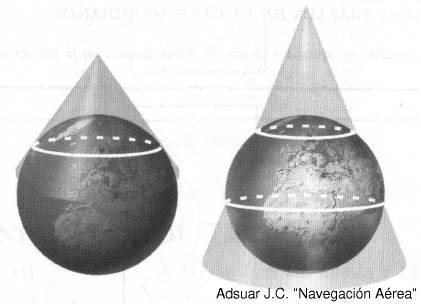
\includegraphics[width=0.45\textwidth]{Imagenes/06.00.navegacion/proy-conicas-tang-sec.png}
% %   \caption{Proyecci\'on c\onica tangente (izquierda) y secante (derecha) \\
% % 	 {\tiny ( fuente:\url{http://nacc.upc.es/cartas/cartas.clas-proy.html})}
% % 	}
% %         \label{fig:proyecciones.conicas.tang.secante}
% % \end{floatingfigure}

% Asimismo, los meridianos deber\'ian indicarse a intervalos de 30', con marcas de graduaci\'on a intervalos de 1', tanto para los paralelos como para los meridianos. Los intervalos de 10' se marcar\'an de manera distintiva.

% La denominaci\'on de esta carta se har\'a (cuando sea aplicable) en funci\'on del n\'umero de referencia de la Carta aeron\'autica mundial - OACI 1:1 000 000 correspondiente, agreg\'andosele una letra que indique a qu\'e cuadrante de la carta mundial corresponde:

% \begin{multicols}{2}
%   \begin{itemize}
%   \item A - Noroeste

%   \item B - Nordeste

%   \item C - Sudeste

%   \item D - Sudoeste
%   \end{itemize}
% \end{multicols}

% Para la carta de ejemplo mencionado arriba (Barcelona, Espa\~na 2319-B), 2319 se refiere a la carta mundial, y la letra B indica el cuadrante nordeste.

% Dada su funci\'on, esta carta tiene que incluir datos topogr\'aficos que tengan importancia para la navegaci\'on visual, as\'i como: Declinaci\'on magn\'etica, espacios \'aereos, obst\'aculos, a\'erodromos y aeropuertos, radioayudas, edificaciones, r\'ios y lagos, autopistas, carreteras, l\'ineas f\'erreas, puntos de referencia (puentes, ruinas, diques, faros, l\'ineas de alta tensi\'on, etc), fronteras, etc. 

% \subsection{Cartas de aproximaci\'on instrumental (IAC = Instrumental Approach Charts)
% }
% \label{sec:cart-de-aproximacion}

% Como su nombre lo indica son cartas donde se esquematiza la aproximaci\'on
% instrumental a una pista determinada de un aeropuerto y en ella se detalla el
% tipo de aproximaci\'on de la que se trata.

% Consta de un encabezado, donde se identifica el aeropuerto, la pista y el tipo
% de aproximaci\'on (NDB, VOR, ILS, etc), en algunas cartas aparecen las letras
% "A" o "B", en este caso no es una aproximaci\'on a la pista, si no solamente
% lleva al avi\'on hasta el aeropuerto y luego este tendr\'a que alinearse con la
% pista, la letra ``A'' corresponde a la primera aproximaci\'on y la ``B'' a la
% segunda.

% \begin{figure}[!htb]
%     \centering
%     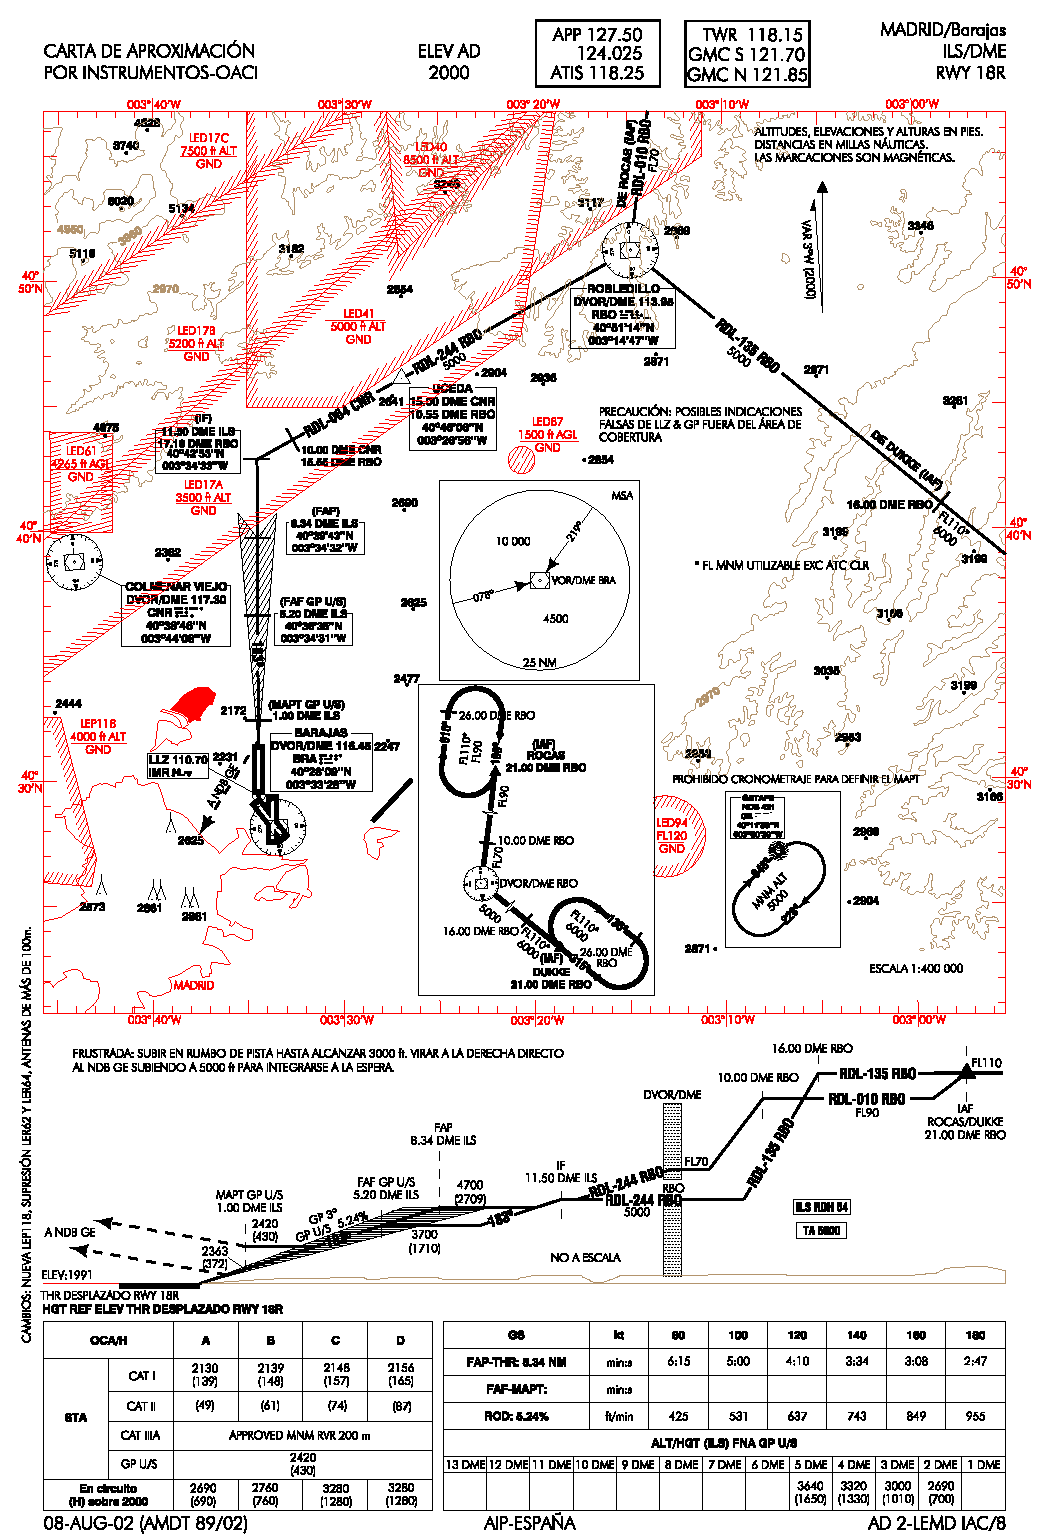
\includegraphics[width=0.85\textwidth]{Imagenes/06.00.navegacion/barajas18r_cropped.pdf}
%     \caption{Carta de aproximaci\'on aeropuerto Barajas (Madrid-Espa\~na), uso
%     did\'actico, orientativo y no usar para un vuelo real, (Fuente: \url{http://www.ultraligero.net/Aproximaciones/aprox.htm})}
%     \label{fig:carta.aproximacion.instrumental.aeropuerto.barajas}
% \end{figure}

% Posee, adem\'as, una vista en planta (vista desde arriba) de la aproximaci\'on en
% donde se detallan todos los rumbos y datos generales de la aproximaci\'on ,
% tambi\'en brinda la informaci\'on de frecuencias, obst\'aculos (en un recuadro
% marcado como MSA), aproximaci\'on fallida, etc.

% Se incluye tambi\'en una vista de perfil de la aproximaci\'on, con informaci\'on
% similar a la anterior pero orientada b\'asicamente hacia los rumbos y altitudes
% a seguir.

% En la parte inferior se encuentra una tabla con los valores m\'inimos operativos
% de aproximaci\'on, los que deber\'an respetarse para cada categor\'ia de nave,
% considerando los sistemas de aproximaci\'on disponibles y basandose en
% condiciones de visibilidad y meteorol\'ogicas.

% Por ultimo puede estar incluido un diagrama de la pista donde se detalla la
% altura sobre el aeropuerto (HAA) y la altura sobre el umbral de la pista (HAT)
% al final de la aproximaci\'on y los obst\'aculos adyacentes de importancia. Se incluye en el diagrama una tabla de tiempos (FAF) utilizados en aproximaciones sin
% precisi\'on.

% Desde luego como en todas las dem\'as cartas pueden estar incluidos detalles de
% elementos de importancia para la maniobra.

% \subsection{Cartas de salida normalizada  (SID = Standar Instrument Departure )}
% \label{sec:cartas-de-salida-normalizada}


% En aeropuertos muy congestionados o con mucho trafico, los controladores
% pueden pedirle a los pilotos que sigan un camino com\'un a todos ellos, para
% evitar tener que explicarle a todos dicha ruta se confeccionan cartas que lo
% explican.

% Similares a las de aproximaci\'on esta cartas constan b\'asicamente de una vista
% en planta (desde arriba) de el camino de salida con las especificaciones
% necesarias, y una segunda secci\'on con la explicaci\'on en forma de texto de
% dicha salida con el detalle y observaciones necesarias y de importancia.

% \subsection{Cartas de llegada normalizada - (STAR - Standar Terminal Arrival Chart)}
% \label{sec:cartas-de-llegada-normalizada}


% Esta carta es similar a la anterior con la salvedad que esta referida a las
% llegadas al aeropuerto en lugar de la salida.

% Esta descripci\'on de cartas esta basada en el sistema cartografico de los EEUU
% conocidas como cartas NOS (National Ocean Service, http://www.nos.noaa.gov )
% departamento dependiente del gobierno de los EEUU.

% Puede haber alguna diferencias con las especificaciones de otros pa\'ises de
% acuerdo a sus necesidades y a la libertad que cada naci\'on posee, aunque el
% criterio es el de estandarizar y pues como en tantos otros aspectos EEUU es el
% referente.

% En la Rep\'ublica Argentina, oficialmente la encargada de producir estas cartas
% es la Fuerza A\'erea Argentina (
% \url{http://www.faa.mil.ar} 
% ), aunque Aerol\'ineas
% Argentinas tambi\'en tiene producci\'on propia.

% Las cartas Jeppesen son producidas por la firma Jeppesen - Sanders
% (
% \url{http://www.jeppesen.com} 
% ) de all\'i el nombre de la carta, dicha empresa
% es capaz de proveer y mantener actualizada la cartograf\'ia de cualquier pa\'is,
% aclarar vale que contienen la misma informaci\'on que las oficiales, los cambios
% principales se basan en la calidad de impresi\'on.

% Todas las cartas no duran eternamente, caducan despu\'es de un tiempo siendo
% responsabilidad del piloto mantenerlas actualizadas.



\subsection{Navegaci\'on Aut\'onoma}
\label{sec:06.navegacion.autonoma}

\subsubsection{Navegaci\'on Observada }%\cite{Aena_SENASA_nav_aerea} }
\label{sec:06.navegacion.observada}

 Es la que se realiza bas\'andose en
referencias del terreno que hay que ver, es una navegaci\'on visual.
Se trata de que el piloto localice las referencias del terreno, para lo
cual es fundamental el uso de buenos 

\begin{minipage}[b]{0.650\linewidth}
	mapas en los que vengan
	reflejados con claridad los accidentes geogr\'aficos, los pueblos y
	ciudades, las carreteras y las v\'ias del ferrocarril, etc. \cite{Aena_SENASA_nav_aerea}

  Para este tipo de navegaci\'on se debe preparar el vuelo,
  estableciendo con toda precisi\'on la ruta que se va a seguir sobre
  el propio mapa.

  En el mismo mapa se marcan puntos en la ruta para dividirla por
  tramos, tratando de que las marcas coincidan con puntos de
  referencia de la ruta. Se deben calcular los tramos por kil\'ometros
  y tiempo que se tarda en volar de un punto a otro.

  Hay que tener buena informaci\'on meteorol\'ogica de toda la ruta y
  llevar la lista de las frecuencias de Torres y Centros de control.
  Si se encontrase perdido, basarse en la \'ultima posici\'on que se
  reconoci\'o y calcular la posici\'on probable por el tiempo
  transcurrido; en esa posici\'on probable tratar de reconocer alguna
  referencia significativa.

\end{minipage}
\begin{minipage}[b]{0.350\linewidth}
	\centering
	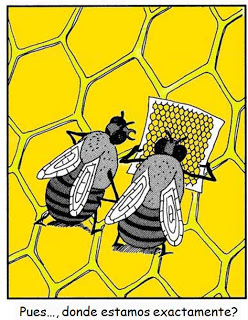
\includegraphics[width=0.9\textwidth]{06.radionavegacion/Imagenes/donde_estamos.jpg}  
\end{minipage}




\section{Navegadores, prestaciones que originan, mediciones presentadas}
\label{sec:U08.01.navegadores.prestaciones}


\section{Navegadores inerciales, plataforma inercial}
\label{sec:U08.navegadores.inerciales}

\begin{flushright}
  Por el Prof. Ing. Pedro Giraudo
\end{flushright}

  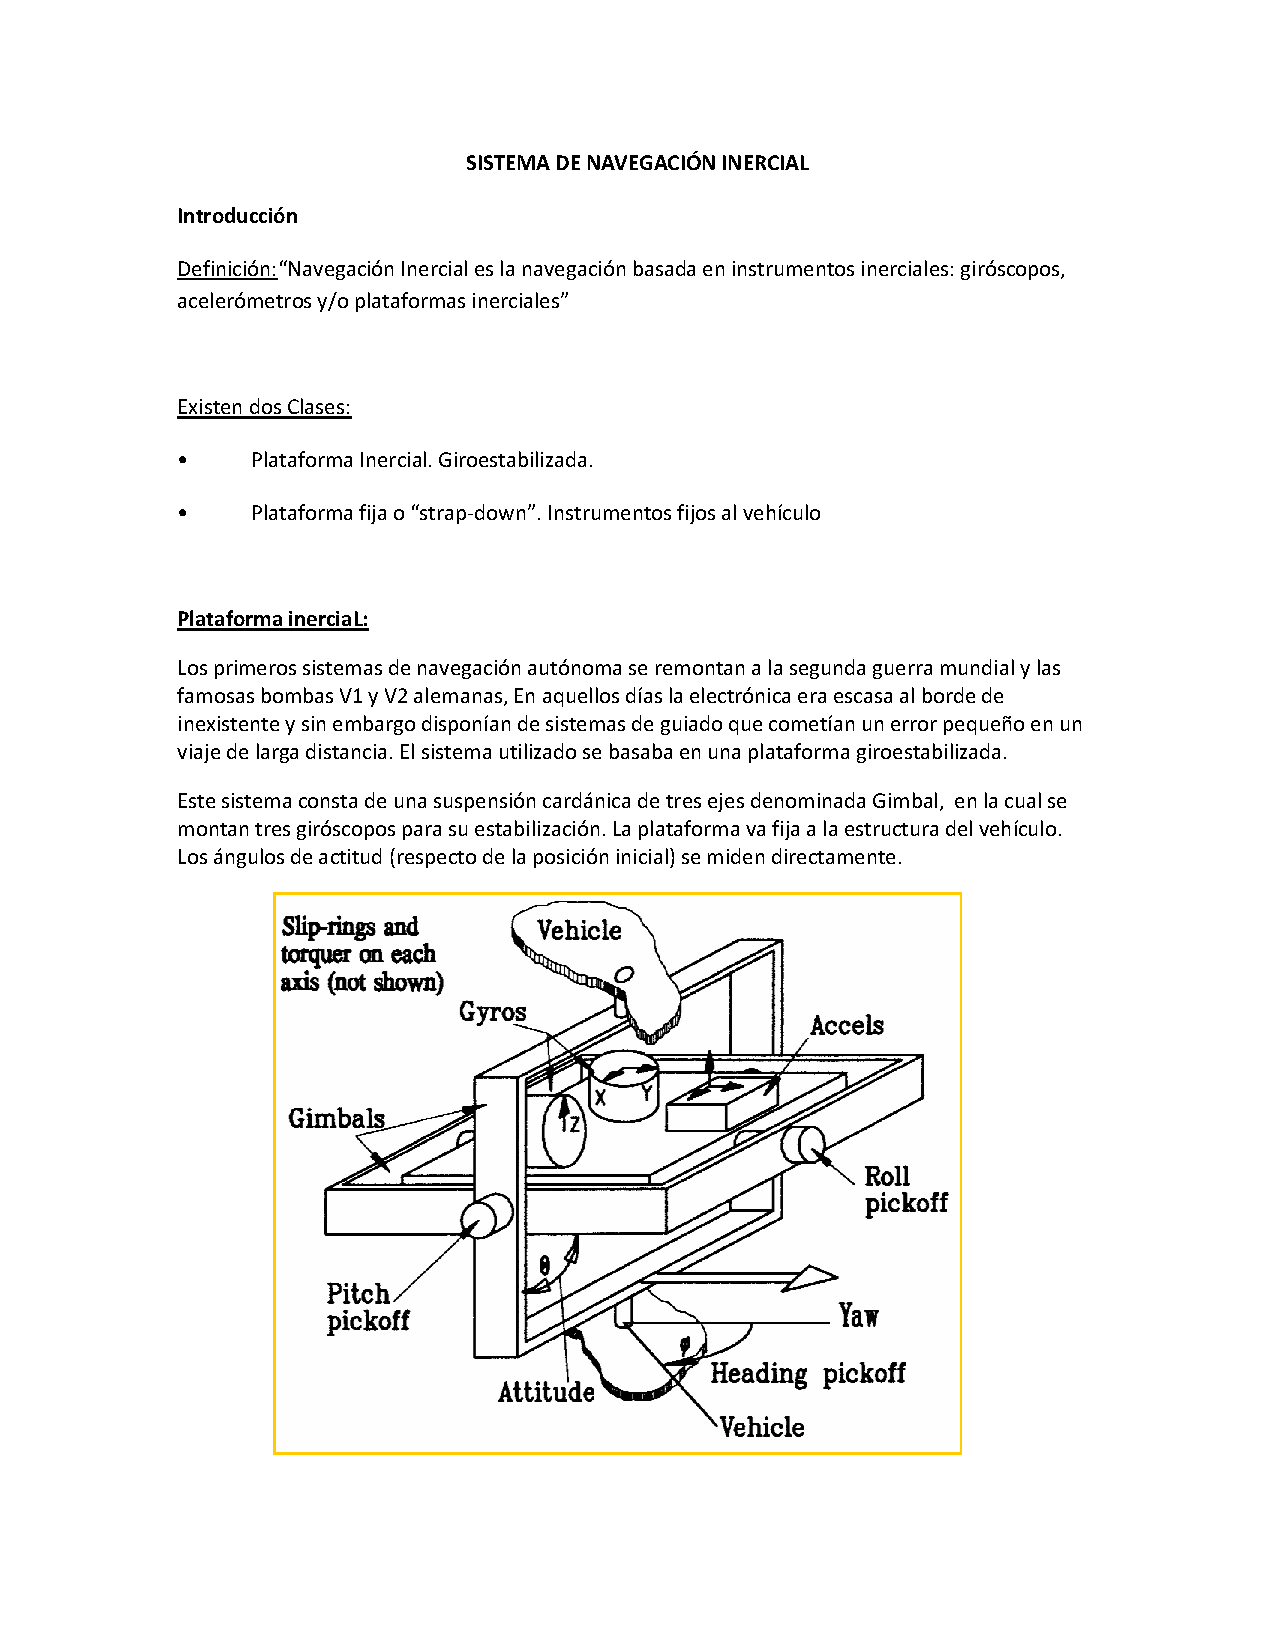
\includepdf[pages=-, fitpaper=false, scale=1.0, %landscape=true,
  offset = 0 -20,
  pagecommand={\thispagestyle{fancy}}]
{08.navegadores/Giraudo.navegacion/INSApunte2020.pdf}



\section{Navegadores GPS}
\label{sec:U08.03.GPS}

\begin{flushright}
  Por el Prof. Ing. Pedro Giraudo
\end{flushright}

  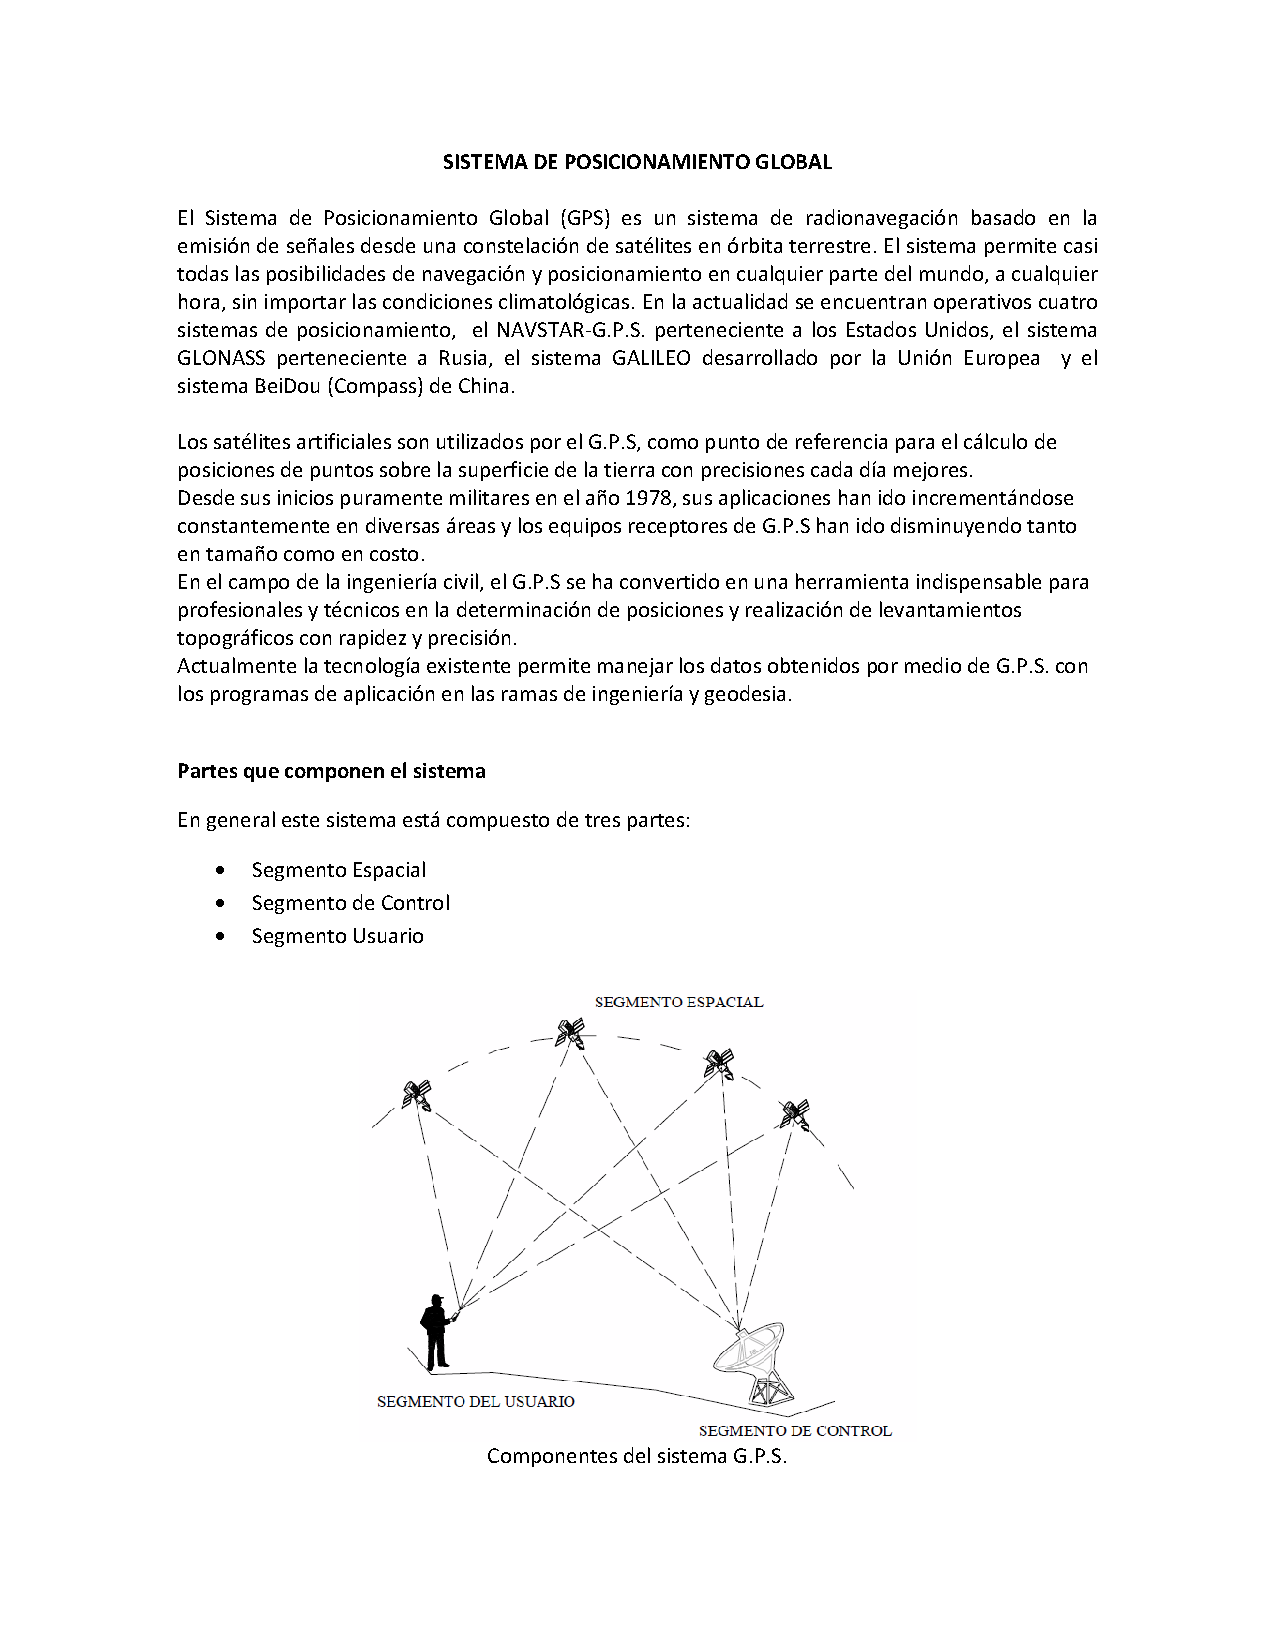
\includepdf[pages=-, fitpaper=false, scale=1.0, %landscape=true,
  offset = 0 -20,
  pagecommand={\thispagestyle{fancy}}]
{08.navegadores/Giraudo.navegacion/GPSApunte2020.pdf}